% =====================================================================
%  Section owner: Joel -- Equilibria, stability and Hopf bifurcation
%  Drop-in file:  % =====================================================================
%  Section owner: Joel -- Equilibria, stability and Hopf bifurcation
%  Drop-in file:  % =====================================================================
%  Section owner: Joel -- Equilibria, stability and Hopf bifurcation
%  Drop-in file:  % =====================================================================
%  Section owner: Joel -- Equilibria, stability and Hopf bifurcation
%  Drop-in file:  \input{joel_stability_section}   (standalone build: joel_main.tex)
%  Needs: amsmath, amssymb, amsthm (theorem, proposition, lemma, remark
%         environments), booktabs, graphicx (PDF companions are used under pdflatex)
%  Figures: graphs/joel_{nullclines,trace_det,regions}.{eps,pdf}
%  Regenerate: python scripts/joel_stability_analysis.py
%  Bibliography keys: in report/references.bib
% =====================================================================

\section{Equilibria, Stability and Hopf Bifurcation}\label{sec:joel}

Throughout this section we analyse the dimensional Rosenzweig--MacArthur model
\begin{equation}\label{eq:rm}
\frac{dH}{dt}= f(H,P) = rH\Bigl(1-\frac{H}{K}\Bigr)-\frac{aHP}{b+H},
\qquad
\frac{dP}{dt}= g(H,P) = \frac{eaHP}{b+H}-mP,
\end{equation}
with all six parameters $r,K,a,b,e,m$ strictly positive, as defined in the model section.
Every stability statement below is tied either to a derivation given here, to a
cited theorem, or to a numerical check; Table~\ref{tab:joel-evidence} at the end of the
section records which is which.

% ---------------------------------------------------------------------
\subsection{Well-posedness: invariance and boundedness}

\begin{lemma}\label{lem:bounded}
The closed quadrant $\{H\ge 0,\,P\ge 0\}$, both coordinate axes, and the open quadrant are
invariant under~\eqref{eq:rm}. Every solution starting in the quadrant is bounded, with
\[
\limsup_{t\to\infty} H(t)\le K,
\qquad
\limsup_{t\to\infty}\bigl(eH(t)+P(t)\bigr)\le \frac{eK(r+m)^2}{4rm}.
\]
\end{lemma}

\begin{proof}
Both right-hand sides factor as $H\cdot(\cdot)$ and $P\cdot(\cdot)$, so $H=0$ and $P=0$ are
invariant lines and, by uniqueness of solutions, no orbit can cross them. Since
$\dot H\le rH(1-H/K)$, comparison with the logistic equation gives $\limsup H\le K$.
For $W=eH+P$ the predation terms cancel:
$\dot W = erH(1-H/K)-mP = eH\bigl(r(1-H/K)+m\bigr)-mW$.
The quadratic $H\bigl(r(1-H/K)+m\bigr)$ is maximised at $H=K(r+m)/(2r)$ with value
$K(r+m)^2/(4r)$, so $\dot W\le eK(r+m)^2/(4r)-mW$ and the bound follows.
\end{proof}

Boundedness is what later allows the Poincar\'e--Bendixson theorem to be used.

% ---------------------------------------------------------------------
\subsection{Equilibria and biological feasibility}

Setting $f=g=0$:
\begin{itemize}
\item $P=0$ in $g=0$ leaves $rH(1-H/K)=0$, giving the \emph{origin} $E_0=(0,0)$ and the
\emph{prey-only} equilibrium $E_1=(K,0)$.
\item $P\neq 0$ requires $eaH/(b+H)=m$, i.e.
\begin{equation}\label{eq:Hstar}
H^*=\frac{mb}{ea-m},
\end{equation}
and then $f=0$ with $H=H^*\neq0$ gives
\begin{equation}\label{eq:Pstar}
P^*=\frac{r}{a}\Bigl(1-\frac{H^*}{K}\Bigr)(b+H^*)
=\frac{ebr\bigl(K(ea-m)-bm\bigr)}{K(ea-m)^2}.
\end{equation}
This is the \emph{coexistence} equilibrium $E^*=(H^*,P^*)$.
\end{itemize}

\begin{proposition}[Feasibility]\label{prop:feasible}
$E_0$ and $E_1$ always lie in the closed quadrant. $E^*$ lies in the open quadrant if and only if
\[
ea>m \quad\text{and}\quad H^*<K
\qquad\Longleftrightarrow\qquad
m<\frac{eaK}{b+K}.
\]
\end{proposition}

\begin{proof}
$H^*>0$ iff $ea>m$. Given this, $P^*>0$ iff $1-H^*/K>0$. Rearranging $mb/(ea-m)<K$
gives $m(b+K)<eaK$.
\end{proof}

\noindent Biologically, $ea$ is the predator's maximal per-capita birth rate (attained when prey is
abundant), so $ea>m$ says lynx can outgrow their mortality at all; $H^*<K$ says the hare
level lynx need to break even is actually reachable by the prey on its own. Note that
$H^*$ does not depend on $r$ or $K$: the prey level at coexistence is set entirely by the
predator.

% ---------------------------------------------------------------------
\subsection{Jacobian}

Differentiating~\eqref{eq:rm},
\begin{equation}\label{eq:jac}
J(H,P)=\begin{pmatrix}
r\Bigl(1-\dfrac{2H}{K}\Bigr)-\dfrac{abP}{(b+H)^2} & -\dfrac{aH}{b+H}\\[2ex]
\dfrac{eabP}{(b+H)^2} & \dfrac{eaH}{b+H}-m
\end{pmatrix}.
\end{equation}
For a planar system, with $\tau=\operatorname{tr}J$ and $\Delta=\det J$, an equilibrium is a
saddle if $\Delta<0$; is asymptotically stable if $\Delta>0,\ \tau<0$; and is unstable if
$\Delta>0,\ \tau>0$. It is a focus when $\tau^2<4\Delta$ and a node when $\tau^2>4\Delta$.

% ---------------------------------------------------------------------
\subsection{Local stability of each equilibrium}

\paragraph{Origin.} $J(E_0)=\operatorname{diag}(r,-m)$, with eigenvalues $r>0$ and $-m<0$.
$E_0$ is \emph{always a saddle}: the $P$-axis is its stable manifold (lynx alone die out) and the
$H$-axis its unstable manifold (hares alone grow). Joint extinction is never an attractor.

\paragraph{Prey-only equilibrium.}
\[
J(E_1)=\begin{pmatrix}-r & -\dfrac{aK}{b+K}\\[1.5ex] 0 & \dfrac{eaK}{b+K}-m\end{pmatrix},
\qquad
\lambda_1=-r,\quad \lambda_2=\frac{eaK}{b+K}-m .
\]
$E_1$ is a stable node when $\lambda_2<0$, i.e.\ exactly when $E^*$ is \emph{not} feasible, and a
saddle when $\lambda_2>0$, i.e.\ exactly when $E^*$ is feasible. At $K=H^*$ the two equilibria
coincide and exchange stability (a transcritical bifurcation). $\lambda_2$ is the invasion rate
of a rare lynx population into a hare population at carrying capacity.

\paragraph{Coexistence equilibrium.}
At $E^*$ the predator equation gives $eaH^*/(b+H^*)=m$, so $J_{22}=0$. Using the prey nullcline,
$aP^*/(b+H^*)=r(1-H^*/K)$, to eliminate $P^*$ from $J_{11}$:
\[
J_{11}=r\Bigl(1-\frac{2H^*}{K}\Bigr)-\frac{b}{b+H^*}\,r\Bigl(1-\frac{H^*}{K}\Bigr)
=\frac{rH^*\,(K-b-2H^*)}{K\,(b+H^*)} .
\]
Hence
\begin{align}
\tau(E^*) &= \frac{rH^*}{K(b+H^*)}\,\bigl(K-K_H\bigr),
\qquad K_H := b+2H^* = \frac{b\,(ea+m)}{ea-m}, \label{eq:trace}\\
\Delta(E^*) &= -J_{12}J_{21} = \frac{aH^*}{b+H^*}\cdot\frac{eabP^*}{(b+H^*)^2}
= \frac{rmb\,(K-H^*)}{K(b+H^*)}. \label{eq:det}
\end{align}

\begin{theorem}[Local stability of $E^*$]\label{thm:local}
Suppose $E^*$ is feasible ($H^*<K$). Then $\Delta(E^*)>0$, so $E^*$ is never a saddle, and
\[
E^* \text{ is locally asymptotically stable if } K<K_H,
\qquad
E^* \text{ is unstable (a repeller) if } K>K_H .
\]
\end{theorem}

\begin{proof}
$\Delta>0$ follows from~\eqref{eq:det} since $K>H^*$. The sign of $\tau$ is the sign of
$K-K_H$ by~\eqref{eq:trace}. Apply the trace--determinant classification.
\end{proof}

\begin{remark}
The intrinsic hare growth rate $r$ appears in $\tau$ and $\Delta$ only as a positive prefactor.
It therefore sets how fast trajectories spiral, but has \emph{no effect} on whether $E^*$ is stable.
Near feasibility ($K$ just above $H^*$), $\Delta\to0$ while $\tau<0$, so $E^*$ is a stable node;
as $K$ increases it becomes a stable focus once $\tau^2<4\Delta$ (at $K\approx42.5$ for the
illustrative parameters of \S\ref{sec:joel-regimes}), so convergence is oscillatory well before
the Hopf point.
\end{remark}

\begin{table}[ht]
\centering
\caption{Equilibria of~\eqref{eq:rm} and their local stability.}
\label{tab:joel-equilibria}
\small
\begin{tabular}{@{}l l l p{0.33\linewidth}@{}}
\toprule
Equilibrium & Feasible when & Eigenvalues / invariants & Type \\
\midrule
$E_0=(0,0)$ & always & $r,\ -m$ & saddle \\[0.5ex]
$E_1=(K,0)$ & always & $-r,\ \tfrac{eaK}{b+K}-m$ & stable node if $K<H^*$ or $ea\le m$; saddle if $K>H^*$\\[0.5ex]
$E^*=(H^*,P^*)$ & $ea>m,\ H^*<K$ & $\tau\propto K-K_H,\ \Delta>0$ & stable if $K<K_H$; unstable if $K>K_H$\\
\bottomrule
\end{tabular}
\end{table}

% ---------------------------------------------------------------------
\subsection{Nullclines and the phase plane}

\paragraph{Prey nullclines ($\dot H=0$):} the $P$-axis $H=0$, and the parabola
\begin{equation}\label{eq:prey-null}
P=\phi(H):=\frac{r}{a}\Bigl(1-\frac{H}{K}\Bigr)(b+H),
\end{equation}
which is concave, vanishes at $H=-b$ and $H=K$, cuts the $P$-axis at $rb/a$, and peaks at
\[
H_{\text{peak}}=\frac{K-b}{2},\qquad \phi(H_{\text{peak}})=\frac{r(K+b)^2}{4aK}.
\]
$\dot H>0$ below the parabola and $\dot H<0$ above it (for $H>0$).

\paragraph{Predator nullclines ($\dot P=0$):} the $H$-axis $P=0$, and the vertical line
$H=H^*$. $\dot P>0$ to the right of $H=H^*$ (enough prey) and $\dot P<0$ to the left.

\paragraph{Flow.} The two interior nullclines divide the open quadrant into four regions.
Starting below the parabola to the right of $H^*$, both species increase; crossing the parabola
hares start to fall while lynx still rise; crossing $H=H^*$ both fall; crossing back below the
parabola hares recover while lynx are still falling. The flow therefore circulates
\emph{counter-clockwise} around $E^*$ in the $(H,P)$ plane, and lynx peaks lag hare peaks.
Near the Hopf point the lag is a quarter-period; it grows with $K$ (numerically, $2.5$ to $4.5$
years for regimes D--F below).

\paragraph{Graphical stability criterion.} Since $K_H=b+2H^*$ is equivalent to
$H^*=(K-b)/2=H_{\text{peak}}$, Theorem~\ref{thm:local} says:
\begin{center}
\emph{$E^*$ is stable if the predator nullcline cuts the prey parabola to the right of its hump,
and unstable if it cuts to the left.}
\end{center}
This is the original Rosenzweig--MacArthur graphical criterion~\cite{rosenzweig1963}. It also
gives the sign of $J_{11}$ directly: $J_{11}=a\,H^*\phi'(H^*)/(b+H^*)$, so a rising nullcline
(left of the hump) means local prey self-amplification ($J_{11}>0$). Figure~\ref{fig:nullclines} shows both cases.

\begin{figure}[ht]
\centering
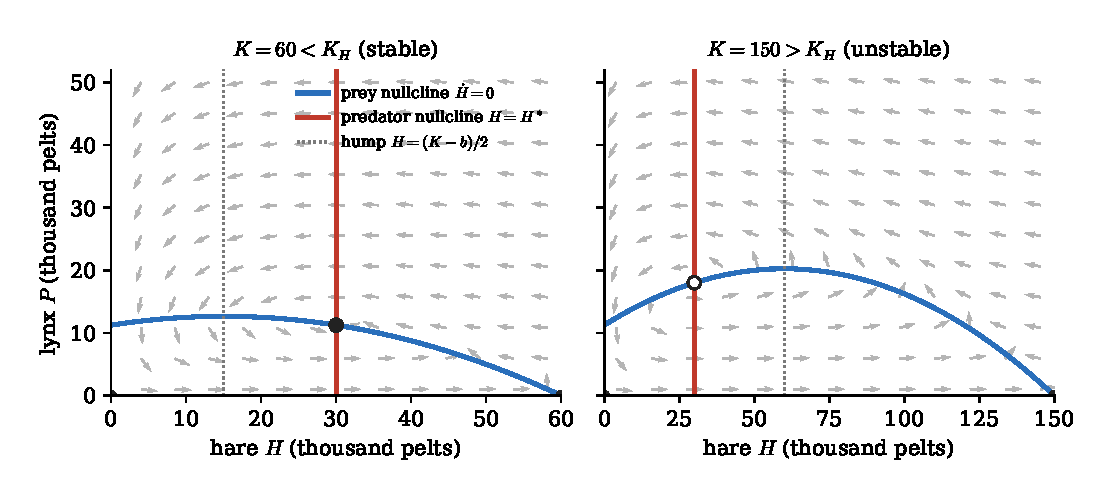
\includegraphics[width=\linewidth]{joel_nullclines}
\caption{Nullclines and direction field for the illustrative parameters
($r=1.5,\ a=4,\ b=30,\ e=0.4,\ m=0.8$; $H^*=30$, $K_H=90$).
Left: $K=60$; the predator nullcline meets the parabola right of its hump and $E^*$ (filled)
is a stable focus. Right: $K=150$; the intersection is left of the hump and $E^*$ (open) is
unstable. Small dots mark $E_0$ and $E_1$.}
\label{fig:nullclines}
\end{figure}

% ---------------------------------------------------------------------
\subsection{Hopf bifurcation with $K$ as the parameter}\label{sec:joel-hopf}

We fix $r,a,b,e,m$ with $ea>m$ and vary $K$ over $(H^*,\infty)$. Note $H^*$ is independent of
$K$, while $P^*$ increases with $K$.

\begin{theorem}[Hopf bifurcation]\label{thm:hopf}
At $K=K_H=b+2H^*$ the coexistence equilibrium undergoes a Hopf bifurcation:
\begin{enumerate}
\item[(i)] $\tau(E^*)=0$ and $\Delta(E^*)=\dfrac{rmb\,(K_H-H^*)}{K_H(b+H^*)}=\dfrac{rmb}{K_H}>0$,
so $J(E^*)$ has eigenvalues $\pm i\omega_0$ with
\[
\omega_0=\sqrt{\frac{rmb}{b+2H^*}},\qquad T_0=\frac{2\pi}{\omega_0};
\]
\item[(ii)] (transversality) the real part of the eigenvalues, $\tau/2$, crosses zero with
nonzero speed:
\[
\frac{d}{dK}\Bigl(\frac{\tau}{2}\Bigr)\Big|_{K=K_H}=\frac{rH^*}{2(b+H^*)(b+2H^*)}>0 .
\]
\end{enumerate}
\end{theorem}

\begin{proof}
(i) Substitute $K=K_H$ into~\eqref{eq:trace} and~\eqref{eq:det}; $K_H-H^*=b+H^*$ simplifies $\Delta$.
(ii) Differentiate~\eqref{eq:trace} in $K$: $\frac{d}{dK}\frac{K-K_H}{K}=\frac{K_H}{K^2}$, which equals
$1/K_H$ at $K=K_H$. All symbolic steps were checked with SymPy (\texttt{scripts/joel\_symbolic\_derivation.py}) and the closed forms are tested against the shared model code (\texttt{tests/test\_stability.py}).
\end{proof}

Conditions (i)--(ii) establish that a pair of complex eigenvalues crosses the imaginary axis.
To conclude that a small periodic orbit is born, and on which side, the Hopf theorem also needs
the first Lyapunov coefficient $\ell_1$ to be nonzero~\cite{kuznetsov2004}: $\ell_1<0$ gives a
\emph{supercritical} bifurcation (a stable cycle for $K>K_H$) and $\ell_1>0$ a subcritical one.

\paragraph{What is analytic and what is numerical.} We separate four statements.
\begin{enumerate}
\item \textbf{Analytic (derived here):} the threshold $K_H$, conditions (i)--(ii), and the
exchange of stability at $E^*$.
\item \textbf{Analytic (derived here): existence of a periodic orbit for $K>K_H$.}
Take any initial condition in the open quadrant. By Lemma~\ref{lem:bounded} its $\omega$-limit
set $\Omega$ is nonempty and compact. $\Omega$ cannot contain $E^*$, which is a repeller.
$\Omega$ cannot be $\{E_1\}$, because the stable manifold of the saddle $E_1$ is the $H$-axis.
If $\Omega$ contained $E_1$ together with other points, it would contain a point of $E_1$'s
stable manifold on the $H$-axis and hence the whole axis orbit through it, which tends backward
to $E_0$; repeating the argument at $E_0$ would put a point of the $P$-axis in $\Omega$, whose
backward orbit is unbounded, contradicting compactness. So $\Omega$ contains no equilibria, and
the Poincar\'e--Bendixson theorem~\cite{strogatz2015} makes $\Omega$ a periodic orbit.
\item \textbf{Cited theorems:} Cheng~\cite{cheng1981} proved the limit cycle is \emph{unique} for
$K>K_H$; since every interior orbit other than $E^*$ tends to a periodic orbit, that unique cycle
attracts them all and is orbitally stable. Hsu~\cite{hsu1978} proved that a locally stable $E^*$
is \emph{globally} stable in the open quadrant whenever the prey nullcline is concave, which our
parabola~\eqref{eq:prey-null} is, so $E^*$ attracts every interior orbit for $H^*<K<K_H$.
We use these results without reproducing their proofs.
\item \textbf{Numerical (for our parameter set only):} evaluating Kuznetsov's formula for
$\ell_1$ at $K=K_H$ gives $\ell_1\approx-4.0\times10^{-4}<0$ (and $-1.3\times10^{-3}$ for a second
set $r=0.7,\ m=0.5,\ b=20$), so the bifurcation is supercritical, consistent with the cited
uniqueness result. Simulations confirm the supercritical signature: the post-transient cycle
half-amplitude in $H$ scales as $(K-K_H)^{1/2}$ (fitted log--log slope $0.507$ for
$K-K_H\in[0.5,8]$), and the period tends to $T_0$.
\end{enumerate}

\noindent None of this says that the \emph{real} hare--lynx data sit on a limit cycle. That
depends on whether fitted parameters satisfy $K>K_H$, and with about two oscillations in
1900--1920 a slowly damped oscillation ($K$ slightly below $K_H$) can fit the same data.
That question belongs to the fitting sections and must be answered there with uncertainty.

\begin{figure}[ht]
\centering
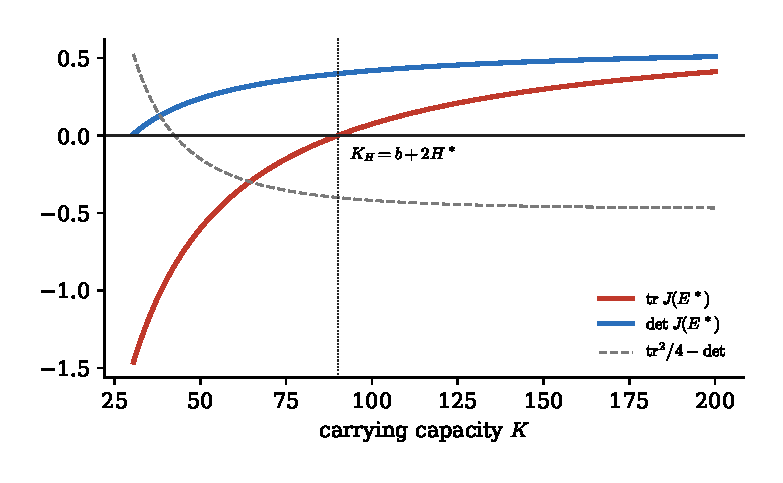
\includegraphics[width=0.7\linewidth]{joel_trace_det}
\caption{Trace and determinant of $J(E^*)$ as functions of $K$ (illustrative parameters).
The determinant stays positive for all feasible $K>H^*=30$, while the trace changes sign at
$K_H=90$. The dashed curve is negative (focus) for $K>42.5$.}
\label{fig:trace-det}
\end{figure}

% ---------------------------------------------------------------------
\subsection{The paradox of enrichment}

Increasing $K$ (enriching the hares' environment) leaves $H^*$ unchanged and only raises $P^*$:
every extra unit of carrying capacity is passed to the predator. Graphically, the prey parabola's
hump $(K-b)/2$ moves right while the predator nullcline stays at $H^*$, so for large enough $K$
the intersection falls left of the hump and the equilibrium destabilises. Past $K_H$ the system
settles on a limit cycle whose amplitude grows with $K$. For our illustrative parameters, at
$K=150$ the hare minimum on the cycle is about $1.1$ thousand, compared with $H^*=30$. In a
finite, stochastic population such deep troughs bring a real risk of extinction. Enrichment
thus \emph{destabilises} the system, the paradox named by Rosenzweig~\cite{rosenzweig1971}.

The mechanism is the saturating Holling type II response. At low $H$ each lynx's consumption
rises almost linearly with prey, which damps fluctuations; near and above $b$ it saturates, so
per-capita predation risk $aP/(b+H)$ \emph{falls} as hares increase. That positive feedback on
prey growth is exactly the term making $J_{11}>0$ left of the hump.

\paragraph{Link to Lotka--Volterra.} In the classical model ($K=\infty$, linear response) the
analogous Jacobian at coexistence has $\tau\equiv0$ for every parameter value, so it sits
permanently on the Hopf boundary. That is why its neutral cycles are structurally unstable: any
small change in the model's form moves it to one side or the other.
Rosenzweig--MacArthur makes the side explicit through the sign of $K-K_H$.

% ---------------------------------------------------------------------
\subsection{Illustrative regimes and numerical validation targets}\label{sec:joel-regimes}

These parameters are \emph{illustrative, not fitted}: $H$ and $P$ in thousands of pelts, $t$ in
years, with $r=1.5,\ a=4,\ b=30,\ e=0.4,\ m=0.8$. Then $ea=1.6=2m$, so $H^*=b=30$, $K_H=90$,
$\omega_0=\sqrt{0.4}\approx0.632$ and $T_0\approx9.94$ years, close to the observed decadal
cycle. Table~\ref{tab:joel-regimes} gives the expected behaviour on each side of the threshold;
the simulation section reproduces these with RK45 (\texttt{rtol}$=10^{-10}$,
\texttt{atol}$=10^{-12}$, 3000-year burn-in, start $(20,5)$).

\begin{table}[ht]
\centering
\small
\caption{Regimes in $K$ (other parameters fixed). Eigenvalues are of $J(E^*)$, except in A where
they are of $J(E_1)$.}
\label{tab:joel-regimes}
\setlength{\tabcolsep}{4pt}
\begin{tabular}{@{}cr l l l@{}}
\toprule
 & $K$ & Linear prediction & Eigenvalues & Long-run behaviour (simulated)\\
\midrule
A & 25  & $E^*$ infeasible ($K<H^*$) & $-1.5,\ -0.073$ & lynx die out; $\to(25,0)$\\
B & 60  & $E^*$ stable focus & $-0.188\pm0.515i$ & $\to(30,\,11.25)$, e-fold $\approx5$ yr\\
C & 85  & just below $K_H$ & $-0.022\pm0.623i$ & $\to(30,\,14.56)$, e-fold $\approx45$ yr\\
D & 90  & Hopf point & $\pm0.632i$ & very slow (algebraic) decay\\
E & 95  & just above $K_H$ & $+0.020\pm0.640i$ & cycle: $H\in[15.8,50.9]$, $P\in[9.8,20.8]$, $T=10.25$\\
F & 150 & well above $K_H$ & $+0.150\pm0.676i$ & cycle: $H\in[1.1,134.3]$, $P\in[1.7,41.2]$, $T=13.91$\\
\bottomrule
\end{tabular}
\end{table}

\noindent Two cautions for the numerics. At D the equilibrium is a weak focus ($\ell_1<0$), so
oscillations decay only like $t^{-1/2}$; after 3000 years the residual amplitude in $H$ is still
about $1.5$, which is expected and is not a sign of a cycle. The cycle at E is already large
because the amplitude coefficient is large ($A_H\approx7.8\sqrt{K-K_H}$), so ``small
amplitude'' only holds within about one unit of $K_H$.

\begin{figure}[ht]
\centering
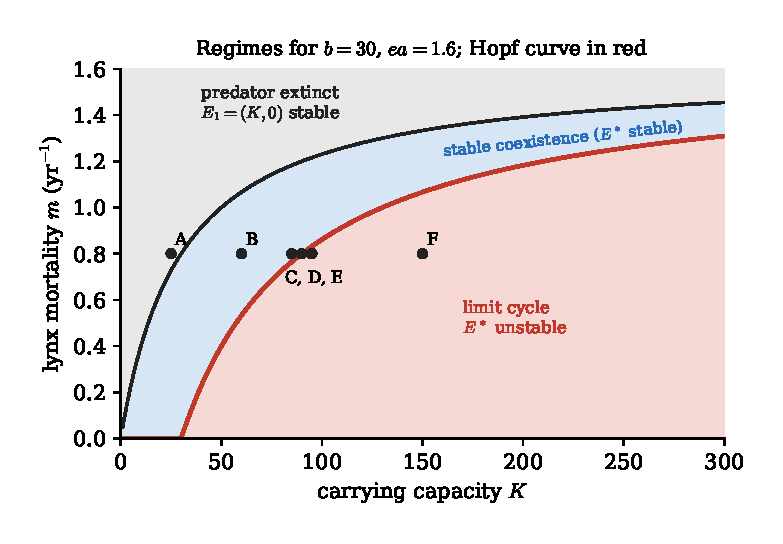
\includegraphics[width=0.7\linewidth]{joel_regions}
\caption{Analytic regimes in the $(K,m)$ plane for $b=30$, $ea=1.6$. Black curve:
$m=eaK/(b+K)$ (predator persistence boundary). Red curve: $m=ea(K-b)/(K+b)$ (Hopf curve).
Dots mark regimes A--F of Table~\ref{tab:joel-regimes}.}
\label{fig:regions}
\end{figure}

% ---------------------------------------------------------------------
\subsection{Sensitivity of the threshold}

Because $K_H=b(ea+m)/(ea-m)$ is explicit, sensitivity can be read off exactly. The elasticities
(percentage change in $K_H$ per percentage change in a parameter) are
\[
\frac{\partial\ln K_H}{\partial\ln b}=1,\qquad
\frac{\partial\ln K_H}{\partial\ln m}=-\frac{\partial\ln K_H}{\partial\ln a}
=-\frac{\partial\ln K_H}{\partial\ln e}=\frac{2\,ea\,m}{(ea)^2-m^2},\qquad
\frac{\partial\ln K_H}{\partial\ln r}=0.
\]
At the illustrative values ($ea=2m$) the middle elasticity is $4/3$: a 10\% rise in lynx
mortality raises the threshold by about 13\%, and so stabilises the system. The elasticity blows
up as $m\to ea$, where the predator is barely viable and $K_H\to\infty$. Weak predators stabilise.

Equivalently, for fixed $K$ the regimes are bands in $m$ (Figure~\ref{fig:regions}):
\[
\underbrace{m<\frac{ea(K-b)}{K+b}}_{\text{limit cycle}}
\qquad
\underbrace{\frac{ea(K-b)}{K+b}<m<\frac{eaK}{K+b}}_{\text{stable coexistence}}
\qquad
\underbrace{m>\frac{eaK}{K+b}}_{\text{lynx extinct}}
\]
A useful single number for any fitted parameter set is the \emph{stability margin}
$\sigma=K/K_H$: $\sigma<1$ means damped oscillations, $\sigma>1$ a limit cycle. Reporting
$\sigma$ (with its spread over fits) is the cleanest way to say whether the data support
sustained cycling.

Two structural facts matter for inference. First, $a$ and $e$ enter $H^*$, $K_H$ and the
stability conditions only through the product $ea$. Second, if lynx are measured only up to an
unknown multiplicative factor $c$ (as pelt counts are), the map $(P,a,e)\mapsto(cP,\,a/c,\,ec)$
leaves~\eqref{eq:rm} unchanged (checked symbolically), so $a$ and $e$ are \emph{not separately
identifiable} from index data. Fitting should fix one of them, or fit $ea$ and a scale, rather
than report both as biological rates.

% ---------------------------------------------------------------------
\subsection{Dimensionless form of the results}

With the scaling $x=H/K$, $y=aP/(rK)$, $s=rt$ (to be reconciled with the frozen scaling in the
model section), \eqref{eq:rm} becomes
\[
x'=x(1-x)-\frac{xy}{\beta+x},\qquad y'=y\Bigl(\frac{\alpha x}{\beta+x}-\delta\Bigr),
\qquad \beta=\frac{b}{K},\ \alpha=\frac{ea}{r},\ \delta=\frac{m}{r}.
\]
Then $x^*=\beta\delta/(\alpha-\delta)$, coexistence requires $\alpha>\delta$ and $x^*<1$, and the
Hopf condition $K=K_H$ reads $\beta(\alpha+\delta)/(\alpha-\delta)=1$, i.e.\ $\beta+2x^*=1$.
Only three combinations of the six parameters control the qualitative dynamics.

% ---------------------------------------------------------------------
\begin{table}[ht]
\centering
\small
\caption{Status of each stability claim in this section.}
\label{tab:joel-evidence}
\begin{tabular}{@{}p{0.52\linewidth}p{0.42\linewidth}@{}}
\toprule
Claim & Evidence \\
\midrule
Equilibria, feasibility, local stability of $E_0,E_1,E^*$ & Derived here; SymPy-checked\\
Hopf threshold $K_H=b+2H^*$, $\Delta>0$, transversality & Derived here; SymPy-checked\\
A periodic orbit exists for every $K>K_H$ & Derived here (Poincar\'e--Bendixson)\\
Cycle is unique and attracting for $K>K_H$ & Cited theorem~\cite{cheng1981}\\
$E^*$ globally stable for $H^*<K<K_H$ & Cited theorem~\cite{hsu1978}\\
Supercritical Hopf ($\ell_1<0$) & Numerical evaluation of analytic formula, two parameter sets\\
$\sqrt{K-K_H}$ amplitude law; periods, amplitudes, lags & Numerical (RK45), illustrative parameters\\
Real hare--lynx data lie on a limit cycle & \emph{Not established here}; requires $\sigma>1$ at fitted values with uncertainty\\
\bottomrule
\end{tabular}
\end{table}
   (standalone build: joel_main.tex)
%  Needs: amsmath, amssymb, amsthm (theorem, proposition, lemma, remark
%         environments), booktabs, graphicx (PDF companions are used under pdflatex)
%  Figures: graphs/joel_{nullclines,trace_det,regions}.{eps,pdf}
%  Regenerate: python scripts/joel_stability_analysis.py
%  Bibliography keys: in report/references.bib
% =====================================================================

\section{Equilibria, Stability and Hopf Bifurcation}\label{sec:joel}

Throughout this section we analyse the dimensional Rosenzweig--MacArthur model
\begin{equation}\label{eq:rm}
\frac{dH}{dt}= f(H,P) = rH\Bigl(1-\frac{H}{K}\Bigr)-\frac{aHP}{b+H},
\qquad
\frac{dP}{dt}= g(H,P) = \frac{eaHP}{b+H}-mP,
\end{equation}
with all six parameters $r,K,a,b,e,m$ strictly positive, as defined in the model section.
Every stability statement below is tied either to a derivation given here, to a
cited theorem, or to a numerical check; Table~\ref{tab:joel-evidence} at the end of the
section records which is which.

% ---------------------------------------------------------------------
\subsection{Well-posedness: invariance and boundedness}

\begin{lemma}\label{lem:bounded}
The closed quadrant $\{H\ge 0,\,P\ge 0\}$, both coordinate axes, and the open quadrant are
invariant under~\eqref{eq:rm}. Every solution starting in the quadrant is bounded, with
\[
\limsup_{t\to\infty} H(t)\le K,
\qquad
\limsup_{t\to\infty}\bigl(eH(t)+P(t)\bigr)\le \frac{eK(r+m)^2}{4rm}.
\]
\end{lemma}

\begin{proof}
Both right-hand sides factor as $H\cdot(\cdot)$ and $P\cdot(\cdot)$, so $H=0$ and $P=0$ are
invariant lines and, by uniqueness of solutions, no orbit can cross them. Since
$\dot H\le rH(1-H/K)$, comparison with the logistic equation gives $\limsup H\le K$.
For $W=eH+P$ the predation terms cancel:
$\dot W = erH(1-H/K)-mP = eH\bigl(r(1-H/K)+m\bigr)-mW$.
The quadratic $H\bigl(r(1-H/K)+m\bigr)$ is maximised at $H=K(r+m)/(2r)$ with value
$K(r+m)^2/(4r)$, so $\dot W\le eK(r+m)^2/(4r)-mW$ and the bound follows.
\end{proof}

Boundedness is what later allows the Poincar\'e--Bendixson theorem to be used.

% ---------------------------------------------------------------------
\subsection{Equilibria and biological feasibility}

Setting $f=g=0$:
\begin{itemize}
\item $P=0$ in $g=0$ leaves $rH(1-H/K)=0$, giving the \emph{origin} $E_0=(0,0)$ and the
\emph{prey-only} equilibrium $E_1=(K,0)$.
\item $P\neq 0$ requires $eaH/(b+H)=m$, i.e.
\begin{equation}\label{eq:Hstar}
H^*=\frac{mb}{ea-m},
\end{equation}
and then $f=0$ with $H=H^*\neq0$ gives
\begin{equation}\label{eq:Pstar}
P^*=\frac{r}{a}\Bigl(1-\frac{H^*}{K}\Bigr)(b+H^*)
=\frac{ebr\bigl(K(ea-m)-bm\bigr)}{K(ea-m)^2}.
\end{equation}
This is the \emph{coexistence} equilibrium $E^*=(H^*,P^*)$.
\end{itemize}

\begin{proposition}[Feasibility]\label{prop:feasible}
$E_0$ and $E_1$ always lie in the closed quadrant. $E^*$ lies in the open quadrant if and only if
\[
ea>m \quad\text{and}\quad H^*<K
\qquad\Longleftrightarrow\qquad
m<\frac{eaK}{b+K}.
\]
\end{proposition}

\begin{proof}
$H^*>0$ iff $ea>m$. Given this, $P^*>0$ iff $1-H^*/K>0$. Rearranging $mb/(ea-m)<K$
gives $m(b+K)<eaK$.
\end{proof}

\noindent Biologically, $ea$ is the predator's maximal per-capita birth rate (attained when prey is
abundant), so $ea>m$ says lynx can outgrow their mortality at all; $H^*<K$ says the hare
level lynx need to break even is actually reachable by the prey on its own. Note that
$H^*$ does not depend on $r$ or $K$: the prey level at coexistence is set entirely by the
predator.

% ---------------------------------------------------------------------
\subsection{Jacobian}

Differentiating~\eqref{eq:rm},
\begin{equation}\label{eq:jac}
J(H,P)=\begin{pmatrix}
r\Bigl(1-\dfrac{2H}{K}\Bigr)-\dfrac{abP}{(b+H)^2} & -\dfrac{aH}{b+H}\\[2ex]
\dfrac{eabP}{(b+H)^2} & \dfrac{eaH}{b+H}-m
\end{pmatrix}.
\end{equation}
For a planar system, with $\tau=\operatorname{tr}J$ and $\Delta=\det J$, an equilibrium is a
saddle if $\Delta<0$; is asymptotically stable if $\Delta>0,\ \tau<0$; and is unstable if
$\Delta>0,\ \tau>0$. It is a focus when $\tau^2<4\Delta$ and a node when $\tau^2>4\Delta$.

% ---------------------------------------------------------------------
\subsection{Local stability of each equilibrium}

\paragraph{Origin.} $J(E_0)=\operatorname{diag}(r,-m)$, with eigenvalues $r>0$ and $-m<0$.
$E_0$ is \emph{always a saddle}: the $P$-axis is its stable manifold (lynx alone die out) and the
$H$-axis its unstable manifold (hares alone grow). Joint extinction is never an attractor.

\paragraph{Prey-only equilibrium.}
\[
J(E_1)=\begin{pmatrix}-r & -\dfrac{aK}{b+K}\\[1.5ex] 0 & \dfrac{eaK}{b+K}-m\end{pmatrix},
\qquad
\lambda_1=-r,\quad \lambda_2=\frac{eaK}{b+K}-m .
\]
$E_1$ is a stable node when $\lambda_2<0$, i.e.\ exactly when $E^*$ is \emph{not} feasible, and a
saddle when $\lambda_2>0$, i.e.\ exactly when $E^*$ is feasible. At $K=H^*$ the two equilibria
coincide and exchange stability (a transcritical bifurcation). $\lambda_2$ is the invasion rate
of a rare lynx population into a hare population at carrying capacity.

\paragraph{Coexistence equilibrium.}
At $E^*$ the predator equation gives $eaH^*/(b+H^*)=m$, so $J_{22}=0$. Using the prey nullcline,
$aP^*/(b+H^*)=r(1-H^*/K)$, to eliminate $P^*$ from $J_{11}$:
\[
J_{11}=r\Bigl(1-\frac{2H^*}{K}\Bigr)-\frac{b}{b+H^*}\,r\Bigl(1-\frac{H^*}{K}\Bigr)
=\frac{rH^*\,(K-b-2H^*)}{K\,(b+H^*)} .
\]
Hence
\begin{align}
\tau(E^*) &= \frac{rH^*}{K(b+H^*)}\,\bigl(K-K_H\bigr),
\qquad K_H := b+2H^* = \frac{b\,(ea+m)}{ea-m}, \label{eq:trace}\\
\Delta(E^*) &= -J_{12}J_{21} = \frac{aH^*}{b+H^*}\cdot\frac{eabP^*}{(b+H^*)^2}
= \frac{rmb\,(K-H^*)}{K(b+H^*)}. \label{eq:det}
\end{align}

\begin{theorem}[Local stability of $E^*$]\label{thm:local}
Suppose $E^*$ is feasible ($H^*<K$). Then $\Delta(E^*)>0$, so $E^*$ is never a saddle, and
\[
E^* \text{ is locally asymptotically stable if } K<K_H,
\qquad
E^* \text{ is unstable (a repeller) if } K>K_H .
\]
\end{theorem}

\begin{proof}
$\Delta>0$ follows from~\eqref{eq:det} since $K>H^*$. The sign of $\tau$ is the sign of
$K-K_H$ by~\eqref{eq:trace}. Apply the trace--determinant classification.
\end{proof}

\begin{remark}
The intrinsic hare growth rate $r$ appears in $\tau$ and $\Delta$ only as a positive prefactor.
It therefore sets how fast trajectories spiral, but has \emph{no effect} on whether $E^*$ is stable.
Near feasibility ($K$ just above $H^*$), $\Delta\to0$ while $\tau<0$, so $E^*$ is a stable node;
as $K$ increases it becomes a stable focus once $\tau^2<4\Delta$ (at $K\approx42.5$ for the
illustrative parameters of \S\ref{sec:joel-regimes}), so convergence is oscillatory well before
the Hopf point.
\end{remark}

\begin{table}[ht]
\centering
\caption{Equilibria of~\eqref{eq:rm} and their local stability.}
\label{tab:joel-equilibria}
\small
\begin{tabular}{@{}l l l p{0.33\linewidth}@{}}
\toprule
Equilibrium & Feasible when & Eigenvalues / invariants & Type \\
\midrule
$E_0=(0,0)$ & always & $r,\ -m$ & saddle \\[0.5ex]
$E_1=(K,0)$ & always & $-r,\ \tfrac{eaK}{b+K}-m$ & stable node if $K<H^*$ or $ea\le m$; saddle if $K>H^*$\\[0.5ex]
$E^*=(H^*,P^*)$ & $ea>m,\ H^*<K$ & $\tau\propto K-K_H,\ \Delta>0$ & stable if $K<K_H$; unstable if $K>K_H$\\
\bottomrule
\end{tabular}
\end{table}

% ---------------------------------------------------------------------
\subsection{Nullclines and the phase plane}

\paragraph{Prey nullclines ($\dot H=0$):} the $P$-axis $H=0$, and the parabola
\begin{equation}\label{eq:prey-null}
P=\phi(H):=\frac{r}{a}\Bigl(1-\frac{H}{K}\Bigr)(b+H),
\end{equation}
which is concave, vanishes at $H=-b$ and $H=K$, cuts the $P$-axis at $rb/a$, and peaks at
\[
H_{\text{peak}}=\frac{K-b}{2},\qquad \phi(H_{\text{peak}})=\frac{r(K+b)^2}{4aK}.
\]
$\dot H>0$ below the parabola and $\dot H<0$ above it (for $H>0$).

\paragraph{Predator nullclines ($\dot P=0$):} the $H$-axis $P=0$, and the vertical line
$H=H^*$. $\dot P>0$ to the right of $H=H^*$ (enough prey) and $\dot P<0$ to the left.

\paragraph{Flow.} The two interior nullclines divide the open quadrant into four regions.
Starting below the parabola to the right of $H^*$, both species increase; crossing the parabola
hares start to fall while lynx still rise; crossing $H=H^*$ both fall; crossing back below the
parabola hares recover while lynx are still falling. The flow therefore circulates
\emph{counter-clockwise} around $E^*$ in the $(H,P)$ plane, and lynx peaks lag hare peaks.
Near the Hopf point the lag is a quarter-period; it grows with $K$ (numerically, $2.5$ to $4.5$
years for regimes D--F below).

\paragraph{Graphical stability criterion.} Since $K_H=b+2H^*$ is equivalent to
$H^*=(K-b)/2=H_{\text{peak}}$, Theorem~\ref{thm:local} says:
\begin{center}
\emph{$E^*$ is stable if the predator nullcline cuts the prey parabola to the right of its hump,
and unstable if it cuts to the left.}
\end{center}
This is the original Rosenzweig--MacArthur graphical criterion~\cite{rosenzweig1963}. It also
gives the sign of $J_{11}$ directly: $J_{11}=a\,H^*\phi'(H^*)/(b+H^*)$, so a rising nullcline
(left of the hump) means local prey self-amplification ($J_{11}>0$). Figure~\ref{fig:nullclines} shows both cases.

\begin{figure}[ht]
\centering
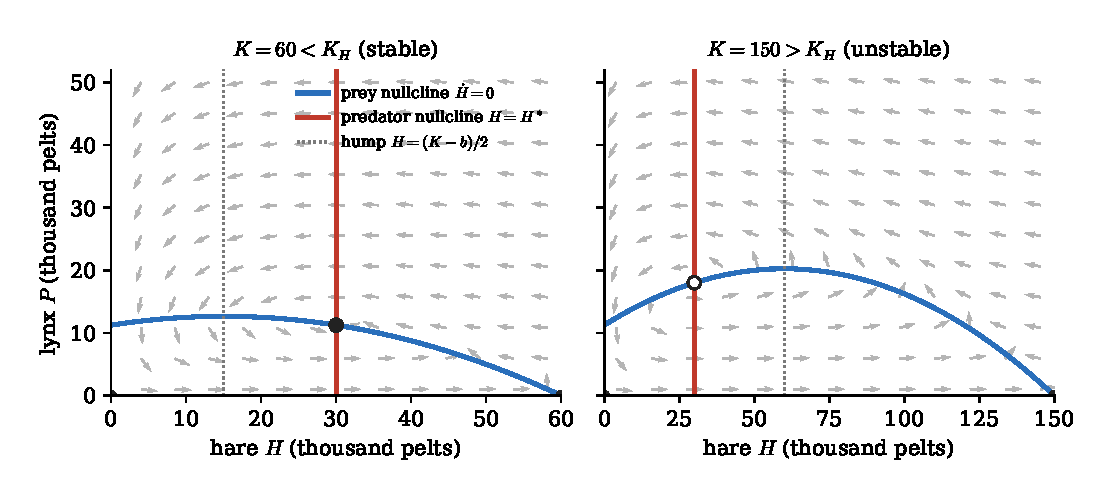
\includegraphics[width=\linewidth]{joel_nullclines}
\caption{Nullclines and direction field for the illustrative parameters
($r=1.5,\ a=4,\ b=30,\ e=0.4,\ m=0.8$; $H^*=30$, $K_H=90$).
Left: $K=60$; the predator nullcline meets the parabola right of its hump and $E^*$ (filled)
is a stable focus. Right: $K=150$; the intersection is left of the hump and $E^*$ (open) is
unstable. Small dots mark $E_0$ and $E_1$.}
\label{fig:nullclines}
\end{figure}

% ---------------------------------------------------------------------
\subsection{Hopf bifurcation with $K$ as the parameter}\label{sec:joel-hopf}

We fix $r,a,b,e,m$ with $ea>m$ and vary $K$ over $(H^*,\infty)$. Note $H^*$ is independent of
$K$, while $P^*$ increases with $K$.

\begin{theorem}[Hopf bifurcation]\label{thm:hopf}
At $K=K_H=b+2H^*$ the coexistence equilibrium undergoes a Hopf bifurcation:
\begin{enumerate}
\item[(i)] $\tau(E^*)=0$ and $\Delta(E^*)=\dfrac{rmb\,(K_H-H^*)}{K_H(b+H^*)}=\dfrac{rmb}{K_H}>0$,
so $J(E^*)$ has eigenvalues $\pm i\omega_0$ with
\[
\omega_0=\sqrt{\frac{rmb}{b+2H^*}},\qquad T_0=\frac{2\pi}{\omega_0};
\]
\item[(ii)] (transversality) the real part of the eigenvalues, $\tau/2$, crosses zero with
nonzero speed:
\[
\frac{d}{dK}\Bigl(\frac{\tau}{2}\Bigr)\Big|_{K=K_H}=\frac{rH^*}{2(b+H^*)(b+2H^*)}>0 .
\]
\end{enumerate}
\end{theorem}

\begin{proof}
(i) Substitute $K=K_H$ into~\eqref{eq:trace} and~\eqref{eq:det}; $K_H-H^*=b+H^*$ simplifies $\Delta$.
(ii) Differentiate~\eqref{eq:trace} in $K$: $\frac{d}{dK}\frac{K-K_H}{K}=\frac{K_H}{K^2}$, which equals
$1/K_H$ at $K=K_H$. All symbolic steps were checked with SymPy (\texttt{scripts/joel\_symbolic\_derivation.py}) and the closed forms are tested against the shared model code (\texttt{tests/test\_stability.py}).
\end{proof}

Conditions (i)--(ii) establish that a pair of complex eigenvalues crosses the imaginary axis.
To conclude that a small periodic orbit is born, and on which side, the Hopf theorem also needs
the first Lyapunov coefficient $\ell_1$ to be nonzero~\cite{kuznetsov2004}: $\ell_1<0$ gives a
\emph{supercritical} bifurcation (a stable cycle for $K>K_H$) and $\ell_1>0$ a subcritical one.

\paragraph{What is analytic and what is numerical.} We separate four statements.
\begin{enumerate}
\item \textbf{Analytic (derived here):} the threshold $K_H$, conditions (i)--(ii), and the
exchange of stability at $E^*$.
\item \textbf{Analytic (derived here): existence of a periodic orbit for $K>K_H$.}
Take any initial condition in the open quadrant. By Lemma~\ref{lem:bounded} its $\omega$-limit
set $\Omega$ is nonempty and compact. $\Omega$ cannot contain $E^*$, which is a repeller.
$\Omega$ cannot be $\{E_1\}$, because the stable manifold of the saddle $E_1$ is the $H$-axis.
If $\Omega$ contained $E_1$ together with other points, it would contain a point of $E_1$'s
stable manifold on the $H$-axis and hence the whole axis orbit through it, which tends backward
to $E_0$; repeating the argument at $E_0$ would put a point of the $P$-axis in $\Omega$, whose
backward orbit is unbounded, contradicting compactness. So $\Omega$ contains no equilibria, and
the Poincar\'e--Bendixson theorem~\cite{strogatz2015} makes $\Omega$ a periodic orbit.
\item \textbf{Cited theorems:} Cheng~\cite{cheng1981} proved the limit cycle is \emph{unique} for
$K>K_H$; since every interior orbit other than $E^*$ tends to a periodic orbit, that unique cycle
attracts them all and is orbitally stable. Hsu~\cite{hsu1978} proved that a locally stable $E^*$
is \emph{globally} stable in the open quadrant whenever the prey nullcline is concave, which our
parabola~\eqref{eq:prey-null} is, so $E^*$ attracts every interior orbit for $H^*<K<K_H$.
We use these results without reproducing their proofs.
\item \textbf{Numerical (for our parameter set only):} evaluating Kuznetsov's formula for
$\ell_1$ at $K=K_H$ gives $\ell_1\approx-4.0\times10^{-4}<0$ (and $-1.3\times10^{-3}$ for a second
set $r=0.7,\ m=0.5,\ b=20$), so the bifurcation is supercritical, consistent with the cited
uniqueness result. Simulations confirm the supercritical signature: the post-transient cycle
half-amplitude in $H$ scales as $(K-K_H)^{1/2}$ (fitted log--log slope $0.507$ for
$K-K_H\in[0.5,8]$), and the period tends to $T_0$.
\end{enumerate}

\noindent None of this says that the \emph{real} hare--lynx data sit on a limit cycle. That
depends on whether fitted parameters satisfy $K>K_H$, and with about two oscillations in
1900--1920 a slowly damped oscillation ($K$ slightly below $K_H$) can fit the same data.
That question belongs to the fitting sections and must be answered there with uncertainty.

\begin{figure}[ht]
\centering
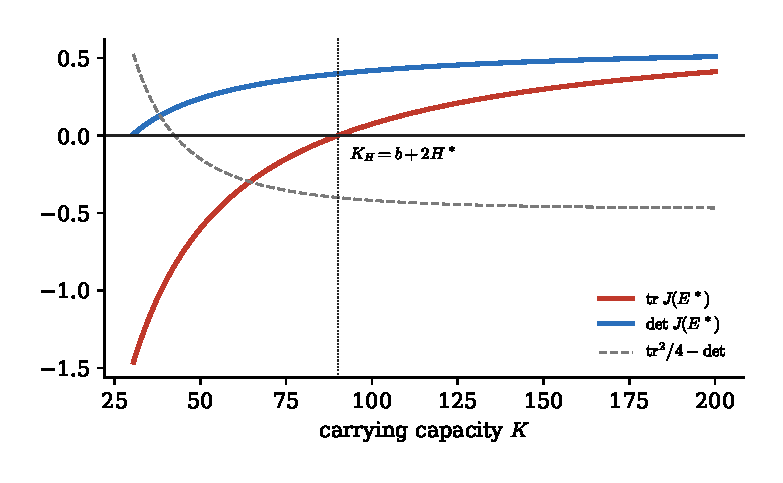
\includegraphics[width=0.7\linewidth]{joel_trace_det}
\caption{Trace and determinant of $J(E^*)$ as functions of $K$ (illustrative parameters).
The determinant stays positive for all feasible $K>H^*=30$, while the trace changes sign at
$K_H=90$. The dashed curve is negative (focus) for $K>42.5$.}
\label{fig:trace-det}
\end{figure}

% ---------------------------------------------------------------------
\subsection{The paradox of enrichment}

Increasing $K$ (enriching the hares' environment) leaves $H^*$ unchanged and only raises $P^*$:
every extra unit of carrying capacity is passed to the predator. Graphically, the prey parabola's
hump $(K-b)/2$ moves right while the predator nullcline stays at $H^*$, so for large enough $K$
the intersection falls left of the hump and the equilibrium destabilises. Past $K_H$ the system
settles on a limit cycle whose amplitude grows with $K$. For our illustrative parameters, at
$K=150$ the hare minimum on the cycle is about $1.1$ thousand, compared with $H^*=30$. In a
finite, stochastic population such deep troughs bring a real risk of extinction. Enrichment
thus \emph{destabilises} the system, the paradox named by Rosenzweig~\cite{rosenzweig1971}.

The mechanism is the saturating Holling type II response. At low $H$ each lynx's consumption
rises almost linearly with prey, which damps fluctuations; near and above $b$ it saturates, so
per-capita predation risk $aP/(b+H)$ \emph{falls} as hares increase. That positive feedback on
prey growth is exactly the term making $J_{11}>0$ left of the hump.

\paragraph{Link to Lotka--Volterra.} In the classical model ($K=\infty$, linear response) the
analogous Jacobian at coexistence has $\tau\equiv0$ for every parameter value, so it sits
permanently on the Hopf boundary. That is why its neutral cycles are structurally unstable: any
small change in the model's form moves it to one side or the other.
Rosenzweig--MacArthur makes the side explicit through the sign of $K-K_H$.

% ---------------------------------------------------------------------
\subsection{Illustrative regimes and numerical validation targets}\label{sec:joel-regimes}

These parameters are \emph{illustrative, not fitted}: $H$ and $P$ in thousands of pelts, $t$ in
years, with $r=1.5,\ a=4,\ b=30,\ e=0.4,\ m=0.8$. Then $ea=1.6=2m$, so $H^*=b=30$, $K_H=90$,
$\omega_0=\sqrt{0.4}\approx0.632$ and $T_0\approx9.94$ years, close to the observed decadal
cycle. Table~\ref{tab:joel-regimes} gives the expected behaviour on each side of the threshold;
the simulation section reproduces these with RK45 (\texttt{rtol}$=10^{-10}$,
\texttt{atol}$=10^{-12}$, 3000-year burn-in, start $(20,5)$).

\begin{table}[ht]
\centering
\small
\caption{Regimes in $K$ (other parameters fixed). Eigenvalues are of $J(E^*)$, except in A where
they are of $J(E_1)$.}
\label{tab:joel-regimes}
\setlength{\tabcolsep}{4pt}
\begin{tabular}{@{}cr l l l@{}}
\toprule
 & $K$ & Linear prediction & Eigenvalues & Long-run behaviour (simulated)\\
\midrule
A & 25  & $E^*$ infeasible ($K<H^*$) & $-1.5,\ -0.073$ & lynx die out; $\to(25,0)$\\
B & 60  & $E^*$ stable focus & $-0.188\pm0.515i$ & $\to(30,\,11.25)$, e-fold $\approx5$ yr\\
C & 85  & just below $K_H$ & $-0.022\pm0.623i$ & $\to(30,\,14.56)$, e-fold $\approx45$ yr\\
D & 90  & Hopf point & $\pm0.632i$ & very slow (algebraic) decay\\
E & 95  & just above $K_H$ & $+0.020\pm0.640i$ & cycle: $H\in[15.8,50.9]$, $P\in[9.8,20.8]$, $T=10.25$\\
F & 150 & well above $K_H$ & $+0.150\pm0.676i$ & cycle: $H\in[1.1,134.3]$, $P\in[1.7,41.2]$, $T=13.91$\\
\bottomrule
\end{tabular}
\end{table}

\noindent Two cautions for the numerics. At D the equilibrium is a weak focus ($\ell_1<0$), so
oscillations decay only like $t^{-1/2}$; after 3000 years the residual amplitude in $H$ is still
about $1.5$, which is expected and is not a sign of a cycle. The cycle at E is already large
because the amplitude coefficient is large ($A_H\approx7.8\sqrt{K-K_H}$), so ``small
amplitude'' only holds within about one unit of $K_H$.

\begin{figure}[ht]
\centering
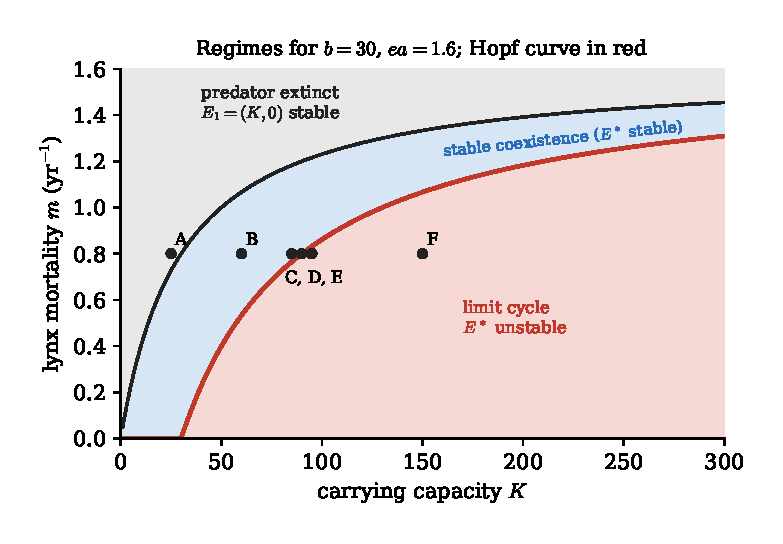
\includegraphics[width=0.7\linewidth]{joel_regions}
\caption{Analytic regimes in the $(K,m)$ plane for $b=30$, $ea=1.6$. Black curve:
$m=eaK/(b+K)$ (predator persistence boundary). Red curve: $m=ea(K-b)/(K+b)$ (Hopf curve).
Dots mark regimes A--F of Table~\ref{tab:joel-regimes}.}
\label{fig:regions}
\end{figure}

% ---------------------------------------------------------------------
\subsection{Sensitivity of the threshold}

Because $K_H=b(ea+m)/(ea-m)$ is explicit, sensitivity can be read off exactly. The elasticities
(percentage change in $K_H$ per percentage change in a parameter) are
\[
\frac{\partial\ln K_H}{\partial\ln b}=1,\qquad
\frac{\partial\ln K_H}{\partial\ln m}=-\frac{\partial\ln K_H}{\partial\ln a}
=-\frac{\partial\ln K_H}{\partial\ln e}=\frac{2\,ea\,m}{(ea)^2-m^2},\qquad
\frac{\partial\ln K_H}{\partial\ln r}=0.
\]
At the illustrative values ($ea=2m$) the middle elasticity is $4/3$: a 10\% rise in lynx
mortality raises the threshold by about 13\%, and so stabilises the system. The elasticity blows
up as $m\to ea$, where the predator is barely viable and $K_H\to\infty$. Weak predators stabilise.

Equivalently, for fixed $K$ the regimes are bands in $m$ (Figure~\ref{fig:regions}):
\[
\underbrace{m<\frac{ea(K-b)}{K+b}}_{\text{limit cycle}}
\qquad
\underbrace{\frac{ea(K-b)}{K+b}<m<\frac{eaK}{K+b}}_{\text{stable coexistence}}
\qquad
\underbrace{m>\frac{eaK}{K+b}}_{\text{lynx extinct}}
\]
A useful single number for any fitted parameter set is the \emph{stability margin}
$\sigma=K/K_H$: $\sigma<1$ means damped oscillations, $\sigma>1$ a limit cycle. Reporting
$\sigma$ (with its spread over fits) is the cleanest way to say whether the data support
sustained cycling.

Two structural facts matter for inference. First, $a$ and $e$ enter $H^*$, $K_H$ and the
stability conditions only through the product $ea$. Second, if lynx are measured only up to an
unknown multiplicative factor $c$ (as pelt counts are), the map $(P,a,e)\mapsto(cP,\,a/c,\,ec)$
leaves~\eqref{eq:rm} unchanged (checked symbolically), so $a$ and $e$ are \emph{not separately
identifiable} from index data. Fitting should fix one of them, or fit $ea$ and a scale, rather
than report both as biological rates.

% ---------------------------------------------------------------------
\subsection{Dimensionless form of the results}

With the scaling $x=H/K$, $y=aP/(rK)$, $s=rt$ (to be reconciled with the frozen scaling in the
model section), \eqref{eq:rm} becomes
\[
x'=x(1-x)-\frac{xy}{\beta+x},\qquad y'=y\Bigl(\frac{\alpha x}{\beta+x}-\delta\Bigr),
\qquad \beta=\frac{b}{K},\ \alpha=\frac{ea}{r},\ \delta=\frac{m}{r}.
\]
Then $x^*=\beta\delta/(\alpha-\delta)$, coexistence requires $\alpha>\delta$ and $x^*<1$, and the
Hopf condition $K=K_H$ reads $\beta(\alpha+\delta)/(\alpha-\delta)=1$, i.e.\ $\beta+2x^*=1$.
Only three combinations of the six parameters control the qualitative dynamics.

% ---------------------------------------------------------------------
\begin{table}[ht]
\centering
\small
\caption{Status of each stability claim in this section.}
\label{tab:joel-evidence}
\begin{tabular}{@{}p{0.52\linewidth}p{0.42\linewidth}@{}}
\toprule
Claim & Evidence \\
\midrule
Equilibria, feasibility, local stability of $E_0,E_1,E^*$ & Derived here; SymPy-checked\\
Hopf threshold $K_H=b+2H^*$, $\Delta>0$, transversality & Derived here; SymPy-checked\\
A periodic orbit exists for every $K>K_H$ & Derived here (Poincar\'e--Bendixson)\\
Cycle is unique and attracting for $K>K_H$ & Cited theorem~\cite{cheng1981}\\
$E^*$ globally stable for $H^*<K<K_H$ & Cited theorem~\cite{hsu1978}\\
Supercritical Hopf ($\ell_1<0$) & Numerical evaluation of analytic formula, two parameter sets\\
$\sqrt{K-K_H}$ amplitude law; periods, amplitudes, lags & Numerical (RK45), illustrative parameters\\
Real hare--lynx data lie on a limit cycle & \emph{Not established here}; requires $\sigma>1$ at fitted values with uncertainty\\
\bottomrule
\end{tabular}
\end{table}
   (standalone build: joel_main.tex)
%  Needs: amsmath, amssymb, amsthm (theorem, proposition, lemma, remark
%         environments), booktabs, graphicx (PDF companions are used under pdflatex)
%  Figures: graphs/joel_{nullclines,trace_det,regions}.{eps,pdf}
%  Regenerate: python scripts/joel_stability_analysis.py
%  Bibliography keys: in report/references.bib
% =====================================================================

\section{Equilibria, Stability and Hopf Bifurcation}\label{sec:joel}

Throughout this section we analyse the dimensional Rosenzweig--MacArthur model
\begin{equation}\label{eq:rm}
\frac{dH}{dt}= f(H,P) = rH\Bigl(1-\frac{H}{K}\Bigr)-\frac{aHP}{b+H},
\qquad
\frac{dP}{dt}= g(H,P) = \frac{eaHP}{b+H}-mP,
\end{equation}
with all six parameters $r,K,a,b,e,m$ strictly positive, as defined in the model section.
Every stability statement below is tied either to a derivation given here, to a
cited theorem, or to a numerical check; Table~\ref{tab:joel-evidence} at the end of the
section records which is which.

% ---------------------------------------------------------------------
\subsection{Well-posedness: invariance and boundedness}

\begin{lemma}\label{lem:bounded}
The closed quadrant $\{H\ge 0,\,P\ge 0\}$, both coordinate axes, and the open quadrant are
invariant under~\eqref{eq:rm}. Every solution starting in the quadrant is bounded, with
\[
\limsup_{t\to\infty} H(t)\le K,
\qquad
\limsup_{t\to\infty}\bigl(eH(t)+P(t)\bigr)\le \frac{eK(r+m)^2}{4rm}.
\]
\end{lemma}

\begin{proof}
Both right-hand sides factor as $H\cdot(\cdot)$ and $P\cdot(\cdot)$, so $H=0$ and $P=0$ are
invariant lines and, by uniqueness of solutions, no orbit can cross them. Since
$\dot H\le rH(1-H/K)$, comparison with the logistic equation gives $\limsup H\le K$.
For $W=eH+P$ the predation terms cancel:
$\dot W = erH(1-H/K)-mP = eH\bigl(r(1-H/K)+m\bigr)-mW$.
The quadratic $H\bigl(r(1-H/K)+m\bigr)$ is maximised at $H=K(r+m)/(2r)$ with value
$K(r+m)^2/(4r)$, so $\dot W\le eK(r+m)^2/(4r)-mW$ and the bound follows.
\end{proof}

Boundedness is what later allows the Poincar\'e--Bendixson theorem to be used.

% ---------------------------------------------------------------------
\subsection{Equilibria and biological feasibility}

Setting $f=g=0$:
\begin{itemize}
\item $P=0$ in $g=0$ leaves $rH(1-H/K)=0$, giving the \emph{origin} $E_0=(0,0)$ and the
\emph{prey-only} equilibrium $E_1=(K,0)$.
\item $P\neq 0$ requires $eaH/(b+H)=m$, i.e.
\begin{equation}\label{eq:Hstar}
H^*=\frac{mb}{ea-m},
\end{equation}
and then $f=0$ with $H=H^*\neq0$ gives
\begin{equation}\label{eq:Pstar}
P^*=\frac{r}{a}\Bigl(1-\frac{H^*}{K}\Bigr)(b+H^*)
=\frac{ebr\bigl(K(ea-m)-bm\bigr)}{K(ea-m)^2}.
\end{equation}
This is the \emph{coexistence} equilibrium $E^*=(H^*,P^*)$.
\end{itemize}

\begin{proposition}[Feasibility]\label{prop:feasible}
$E_0$ and $E_1$ always lie in the closed quadrant. $E^*$ lies in the open quadrant if and only if
\[
ea>m \quad\text{and}\quad H^*<K
\qquad\Longleftrightarrow\qquad
m<\frac{eaK}{b+K}.
\]
\end{proposition}

\begin{proof}
$H^*>0$ iff $ea>m$. Given this, $P^*>0$ iff $1-H^*/K>0$. Rearranging $mb/(ea-m)<K$
gives $m(b+K)<eaK$.
\end{proof}

\noindent Biologically, $ea$ is the predator's maximal per-capita birth rate (attained when prey is
abundant), so $ea>m$ says lynx can outgrow their mortality at all; $H^*<K$ says the hare
level lynx need to break even is actually reachable by the prey on its own. Note that
$H^*$ does not depend on $r$ or $K$: the prey level at coexistence is set entirely by the
predator.

% ---------------------------------------------------------------------
\subsection{Jacobian}

Differentiating~\eqref{eq:rm},
\begin{equation}\label{eq:jac}
J(H,P)=\begin{pmatrix}
r\Bigl(1-\dfrac{2H}{K}\Bigr)-\dfrac{abP}{(b+H)^2} & -\dfrac{aH}{b+H}\\[2ex]
\dfrac{eabP}{(b+H)^2} & \dfrac{eaH}{b+H}-m
\end{pmatrix}.
\end{equation}
For a planar system, with $\tau=\operatorname{tr}J$ and $\Delta=\det J$, an equilibrium is a
saddle if $\Delta<0$; is asymptotically stable if $\Delta>0,\ \tau<0$; and is unstable if
$\Delta>0,\ \tau>0$. It is a focus when $\tau^2<4\Delta$ and a node when $\tau^2>4\Delta$.

% ---------------------------------------------------------------------
\subsection{Local stability of each equilibrium}

\paragraph{Origin.} $J(E_0)=\operatorname{diag}(r,-m)$, with eigenvalues $r>0$ and $-m<0$.
$E_0$ is \emph{always a saddle}: the $P$-axis is its stable manifold (lynx alone die out) and the
$H$-axis its unstable manifold (hares alone grow). Joint extinction is never an attractor.

\paragraph{Prey-only equilibrium.}
\[
J(E_1)=\begin{pmatrix}-r & -\dfrac{aK}{b+K}\\[1.5ex] 0 & \dfrac{eaK}{b+K}-m\end{pmatrix},
\qquad
\lambda_1=-r,\quad \lambda_2=\frac{eaK}{b+K}-m .
\]
$E_1$ is a stable node when $\lambda_2<0$, i.e.\ exactly when $E^*$ is \emph{not} feasible, and a
saddle when $\lambda_2>0$, i.e.\ exactly when $E^*$ is feasible. At $K=H^*$ the two equilibria
coincide and exchange stability (a transcritical bifurcation). $\lambda_2$ is the invasion rate
of a rare lynx population into a hare population at carrying capacity.

\paragraph{Coexistence equilibrium.}
At $E^*$ the predator equation gives $eaH^*/(b+H^*)=m$, so $J_{22}=0$. Using the prey nullcline,
$aP^*/(b+H^*)=r(1-H^*/K)$, to eliminate $P^*$ from $J_{11}$:
\[
J_{11}=r\Bigl(1-\frac{2H^*}{K}\Bigr)-\frac{b}{b+H^*}\,r\Bigl(1-\frac{H^*}{K}\Bigr)
=\frac{rH^*\,(K-b-2H^*)}{K\,(b+H^*)} .
\]
Hence
\begin{align}
\tau(E^*) &= \frac{rH^*}{K(b+H^*)}\,\bigl(K-K_H\bigr),
\qquad K_H := b+2H^* = \frac{b\,(ea+m)}{ea-m}, \label{eq:trace}\\
\Delta(E^*) &= -J_{12}J_{21} = \frac{aH^*}{b+H^*}\cdot\frac{eabP^*}{(b+H^*)^2}
= \frac{rmb\,(K-H^*)}{K(b+H^*)}. \label{eq:det}
\end{align}

\begin{theorem}[Local stability of $E^*$]\label{thm:local}
Suppose $E^*$ is feasible ($H^*<K$). Then $\Delta(E^*)>0$, so $E^*$ is never a saddle, and
\[
E^* \text{ is locally asymptotically stable if } K<K_H,
\qquad
E^* \text{ is unstable (a repeller) if } K>K_H .
\]
\end{theorem}

\begin{proof}
$\Delta>0$ follows from~\eqref{eq:det} since $K>H^*$. The sign of $\tau$ is the sign of
$K-K_H$ by~\eqref{eq:trace}. Apply the trace--determinant classification.
\end{proof}

\begin{remark}
The intrinsic hare growth rate $r$ appears in $\tau$ and $\Delta$ only as a positive prefactor.
It therefore sets how fast trajectories spiral, but has \emph{no effect} on whether $E^*$ is stable.
Near feasibility ($K$ just above $H^*$), $\Delta\to0$ while $\tau<0$, so $E^*$ is a stable node;
as $K$ increases it becomes a stable focus once $\tau^2<4\Delta$ (at $K\approx42.5$ for the
illustrative parameters of \S\ref{sec:joel-regimes}), so convergence is oscillatory well before
the Hopf point.
\end{remark}

\begin{table}[ht]
\centering
\caption{Equilibria of~\eqref{eq:rm} and their local stability.}
\label{tab:joel-equilibria}
\small
\begin{tabular}{@{}l l l p{0.33\linewidth}@{}}
\toprule
Equilibrium & Feasible when & Eigenvalues / invariants & Type \\
\midrule
$E_0=(0,0)$ & always & $r,\ -m$ & saddle \\[0.5ex]
$E_1=(K,0)$ & always & $-r,\ \tfrac{eaK}{b+K}-m$ & stable node if $K<H^*$ or $ea\le m$; saddle if $K>H^*$\\[0.5ex]
$E^*=(H^*,P^*)$ & $ea>m,\ H^*<K$ & $\tau\propto K-K_H,\ \Delta>0$ & stable if $K<K_H$; unstable if $K>K_H$\\
\bottomrule
\end{tabular}
\end{table}

% ---------------------------------------------------------------------
\subsection{Nullclines and the phase plane}

\paragraph{Prey nullclines ($\dot H=0$):} the $P$-axis $H=0$, and the parabola
\begin{equation}\label{eq:prey-null}
P=\phi(H):=\frac{r}{a}\Bigl(1-\frac{H}{K}\Bigr)(b+H),
\end{equation}
which is concave, vanishes at $H=-b$ and $H=K$, cuts the $P$-axis at $rb/a$, and peaks at
\[
H_{\text{peak}}=\frac{K-b}{2},\qquad \phi(H_{\text{peak}})=\frac{r(K+b)^2}{4aK}.
\]
$\dot H>0$ below the parabola and $\dot H<0$ above it (for $H>0$).

\paragraph{Predator nullclines ($\dot P=0$):} the $H$-axis $P=0$, and the vertical line
$H=H^*$. $\dot P>0$ to the right of $H=H^*$ (enough prey) and $\dot P<0$ to the left.

\paragraph{Flow.} The two interior nullclines divide the open quadrant into four regions.
Starting below the parabola to the right of $H^*$, both species increase; crossing the parabola
hares start to fall while lynx still rise; crossing $H=H^*$ both fall; crossing back below the
parabola hares recover while lynx are still falling. The flow therefore circulates
\emph{counter-clockwise} around $E^*$ in the $(H,P)$ plane, and lynx peaks lag hare peaks.
Near the Hopf point the lag is a quarter-period; it grows with $K$ (numerically, $2.5$ to $4.5$
years for regimes D--F below).

\paragraph{Graphical stability criterion.} Since $K_H=b+2H^*$ is equivalent to
$H^*=(K-b)/2=H_{\text{peak}}$, Theorem~\ref{thm:local} says:
\begin{center}
\emph{$E^*$ is stable if the predator nullcline cuts the prey parabola to the right of its hump,
and unstable if it cuts to the left.}
\end{center}
This is the original Rosenzweig--MacArthur graphical criterion~\cite{rosenzweig1963}. It also
gives the sign of $J_{11}$ directly: $J_{11}=a\,H^*\phi'(H^*)/(b+H^*)$, so a rising nullcline
(left of the hump) means local prey self-amplification ($J_{11}>0$). Figure~\ref{fig:nullclines} shows both cases.

\begin{figure}[ht]
\centering
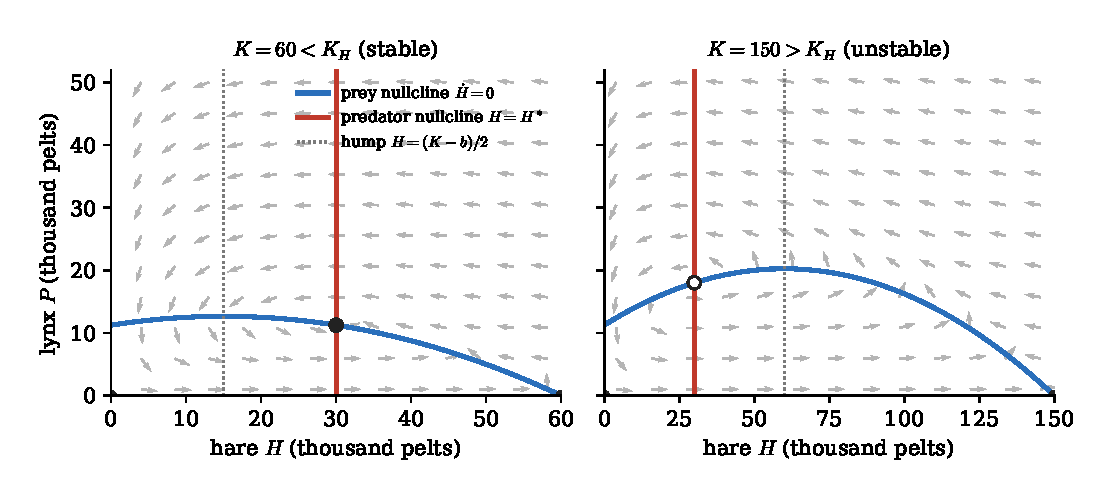
\includegraphics[width=\linewidth]{joel_nullclines}
\caption{Nullclines and direction field for the illustrative parameters
($r=1.5,\ a=4,\ b=30,\ e=0.4,\ m=0.8$; $H^*=30$, $K_H=90$).
Left: $K=60$; the predator nullcline meets the parabola right of its hump and $E^*$ (filled)
is a stable focus. Right: $K=150$; the intersection is left of the hump and $E^*$ (open) is
unstable. Small dots mark $E_0$ and $E_1$.}
\label{fig:nullclines}
\end{figure}

% ---------------------------------------------------------------------
\subsection{Hopf bifurcation with $K$ as the parameter}\label{sec:joel-hopf}

We fix $r,a,b,e,m$ with $ea>m$ and vary $K$ over $(H^*,\infty)$. Note $H^*$ is independent of
$K$, while $P^*$ increases with $K$.

\begin{theorem}[Hopf bifurcation]\label{thm:hopf}
At $K=K_H=b+2H^*$ the coexistence equilibrium undergoes a Hopf bifurcation:
\begin{enumerate}
\item[(i)] $\tau(E^*)=0$ and $\Delta(E^*)=\dfrac{rmb\,(K_H-H^*)}{K_H(b+H^*)}=\dfrac{rmb}{K_H}>0$,
so $J(E^*)$ has eigenvalues $\pm i\omega_0$ with
\[
\omega_0=\sqrt{\frac{rmb}{b+2H^*}},\qquad T_0=\frac{2\pi}{\omega_0};
\]
\item[(ii)] (transversality) the real part of the eigenvalues, $\tau/2$, crosses zero with
nonzero speed:
\[
\frac{d}{dK}\Bigl(\frac{\tau}{2}\Bigr)\Big|_{K=K_H}=\frac{rH^*}{2(b+H^*)(b+2H^*)}>0 .
\]
\end{enumerate}
\end{theorem}

\begin{proof}
(i) Substitute $K=K_H$ into~\eqref{eq:trace} and~\eqref{eq:det}; $K_H-H^*=b+H^*$ simplifies $\Delta$.
(ii) Differentiate~\eqref{eq:trace} in $K$: $\frac{d}{dK}\frac{K-K_H}{K}=\frac{K_H}{K^2}$, which equals
$1/K_H$ at $K=K_H$. All symbolic steps were checked with SymPy (\texttt{scripts/joel\_symbolic\_derivation.py}) and the closed forms are tested against the shared model code (\texttt{tests/test\_stability.py}).
\end{proof}

Conditions (i)--(ii) establish that a pair of complex eigenvalues crosses the imaginary axis.
To conclude that a small periodic orbit is born, and on which side, the Hopf theorem also needs
the first Lyapunov coefficient $\ell_1$ to be nonzero~\cite{kuznetsov2004}: $\ell_1<0$ gives a
\emph{supercritical} bifurcation (a stable cycle for $K>K_H$) and $\ell_1>0$ a subcritical one.

\paragraph{What is analytic and what is numerical.} We separate four statements.
\begin{enumerate}
\item \textbf{Analytic (derived here):} the threshold $K_H$, conditions (i)--(ii), and the
exchange of stability at $E^*$.
\item \textbf{Analytic (derived here): existence of a periodic orbit for $K>K_H$.}
Take any initial condition in the open quadrant. By Lemma~\ref{lem:bounded} its $\omega$-limit
set $\Omega$ is nonempty and compact. $\Omega$ cannot contain $E^*$, which is a repeller.
$\Omega$ cannot be $\{E_1\}$, because the stable manifold of the saddle $E_1$ is the $H$-axis.
If $\Omega$ contained $E_1$ together with other points, it would contain a point of $E_1$'s
stable manifold on the $H$-axis and hence the whole axis orbit through it, which tends backward
to $E_0$; repeating the argument at $E_0$ would put a point of the $P$-axis in $\Omega$, whose
backward orbit is unbounded, contradicting compactness. So $\Omega$ contains no equilibria, and
the Poincar\'e--Bendixson theorem~\cite{strogatz2015} makes $\Omega$ a periodic orbit.
\item \textbf{Cited theorems:} Cheng~\cite{cheng1981} proved the limit cycle is \emph{unique} for
$K>K_H$; since every interior orbit other than $E^*$ tends to a periodic orbit, that unique cycle
attracts them all and is orbitally stable. Hsu~\cite{hsu1978} proved that a locally stable $E^*$
is \emph{globally} stable in the open quadrant whenever the prey nullcline is concave, which our
parabola~\eqref{eq:prey-null} is, so $E^*$ attracts every interior orbit for $H^*<K<K_H$.
We use these results without reproducing their proofs.
\item \textbf{Numerical (for our parameter set only):} evaluating Kuznetsov's formula for
$\ell_1$ at $K=K_H$ gives $\ell_1\approx-4.0\times10^{-4}<0$ (and $-1.3\times10^{-3}$ for a second
set $r=0.7,\ m=0.5,\ b=20$), so the bifurcation is supercritical, consistent with the cited
uniqueness result. Simulations confirm the supercritical signature: the post-transient cycle
half-amplitude in $H$ scales as $(K-K_H)^{1/2}$ (fitted log--log slope $0.507$ for
$K-K_H\in[0.5,8]$), and the period tends to $T_0$.
\end{enumerate}

\noindent None of this says that the \emph{real} hare--lynx data sit on a limit cycle. That
depends on whether fitted parameters satisfy $K>K_H$, and with about two oscillations in
1900--1920 a slowly damped oscillation ($K$ slightly below $K_H$) can fit the same data.
That question belongs to the fitting sections and must be answered there with uncertainty.

\begin{figure}[ht]
\centering
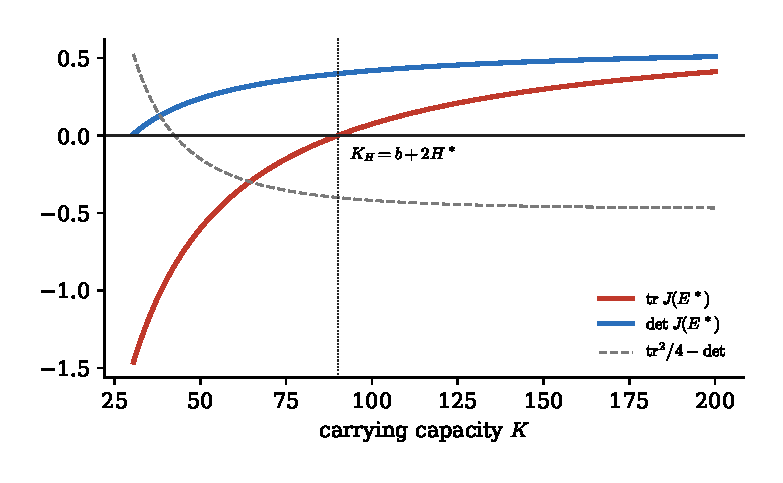
\includegraphics[width=0.7\linewidth]{joel_trace_det}
\caption{Trace and determinant of $J(E^*)$ as functions of $K$ (illustrative parameters).
The determinant stays positive for all feasible $K>H^*=30$, while the trace changes sign at
$K_H=90$. The dashed curve is negative (focus) for $K>42.5$.}
\label{fig:trace-det}
\end{figure}

% ---------------------------------------------------------------------
\subsection{The paradox of enrichment}

Increasing $K$ (enriching the hares' environment) leaves $H^*$ unchanged and only raises $P^*$:
every extra unit of carrying capacity is passed to the predator. Graphically, the prey parabola's
hump $(K-b)/2$ moves right while the predator nullcline stays at $H^*$, so for large enough $K$
the intersection falls left of the hump and the equilibrium destabilises. Past $K_H$ the system
settles on a limit cycle whose amplitude grows with $K$. For our illustrative parameters, at
$K=150$ the hare minimum on the cycle is about $1.1$ thousand, compared with $H^*=30$. In a
finite, stochastic population such deep troughs bring a real risk of extinction. Enrichment
thus \emph{destabilises} the system, the paradox named by Rosenzweig~\cite{rosenzweig1971}.

The mechanism is the saturating Holling type II response. At low $H$ each lynx's consumption
rises almost linearly with prey, which damps fluctuations; near and above $b$ it saturates, so
per-capita predation risk $aP/(b+H)$ \emph{falls} as hares increase. That positive feedback on
prey growth is exactly the term making $J_{11}>0$ left of the hump.

\paragraph{Link to Lotka--Volterra.} In the classical model ($K=\infty$, linear response) the
analogous Jacobian at coexistence has $\tau\equiv0$ for every parameter value, so it sits
permanently on the Hopf boundary. That is why its neutral cycles are structurally unstable: any
small change in the model's form moves it to one side or the other.
Rosenzweig--MacArthur makes the side explicit through the sign of $K-K_H$.

% ---------------------------------------------------------------------
\subsection{Illustrative regimes and numerical validation targets}\label{sec:joel-regimes}

These parameters are \emph{illustrative, not fitted}: $H$ and $P$ in thousands of pelts, $t$ in
years, with $r=1.5,\ a=4,\ b=30,\ e=0.4,\ m=0.8$. Then $ea=1.6=2m$, so $H^*=b=30$, $K_H=90$,
$\omega_0=\sqrt{0.4}\approx0.632$ and $T_0\approx9.94$ years, close to the observed decadal
cycle. Table~\ref{tab:joel-regimes} gives the expected behaviour on each side of the threshold;
the simulation section reproduces these with RK45 (\texttt{rtol}$=10^{-10}$,
\texttt{atol}$=10^{-12}$, 3000-year burn-in, start $(20,5)$).

\begin{table}[ht]
\centering
\small
\caption{Regimes in $K$ (other parameters fixed). Eigenvalues are of $J(E^*)$, except in A where
they are of $J(E_1)$.}
\label{tab:joel-regimes}
\setlength{\tabcolsep}{4pt}
\begin{tabular}{@{}cr l l l@{}}
\toprule
 & $K$ & Linear prediction & Eigenvalues & Long-run behaviour (simulated)\\
\midrule
A & 25  & $E^*$ infeasible ($K<H^*$) & $-1.5,\ -0.073$ & lynx die out; $\to(25,0)$\\
B & 60  & $E^*$ stable focus & $-0.188\pm0.515i$ & $\to(30,\,11.25)$, e-fold $\approx5$ yr\\
C & 85  & just below $K_H$ & $-0.022\pm0.623i$ & $\to(30,\,14.56)$, e-fold $\approx45$ yr\\
D & 90  & Hopf point & $\pm0.632i$ & very slow (algebraic) decay\\
E & 95  & just above $K_H$ & $+0.020\pm0.640i$ & cycle: $H\in[15.8,50.9]$, $P\in[9.8,20.8]$, $T=10.25$\\
F & 150 & well above $K_H$ & $+0.150\pm0.676i$ & cycle: $H\in[1.1,134.3]$, $P\in[1.7,41.2]$, $T=13.91$\\
\bottomrule
\end{tabular}
\end{table}

\noindent Two cautions for the numerics. At D the equilibrium is a weak focus ($\ell_1<0$), so
oscillations decay only like $t^{-1/2}$; after 3000 years the residual amplitude in $H$ is still
about $1.5$, which is expected and is not a sign of a cycle. The cycle at E is already large
because the amplitude coefficient is large ($A_H\approx7.8\sqrt{K-K_H}$), so ``small
amplitude'' only holds within about one unit of $K_H$.

\begin{figure}[ht]
\centering
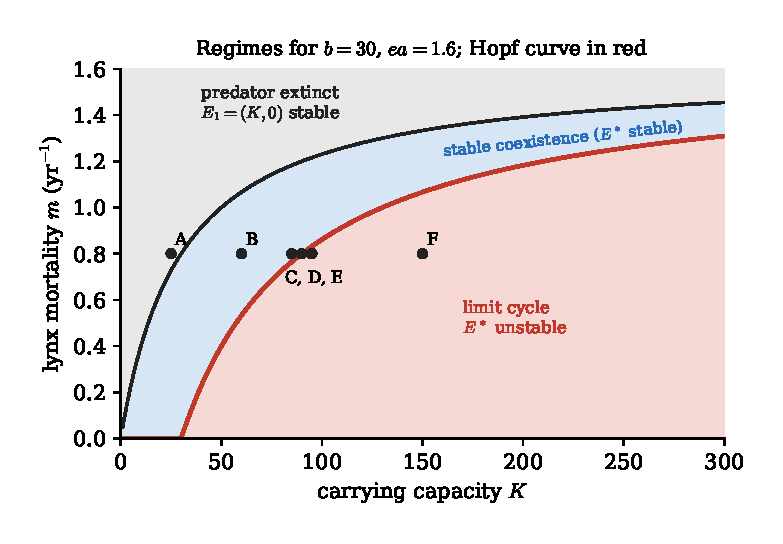
\includegraphics[width=0.7\linewidth]{joel_regions}
\caption{Analytic regimes in the $(K,m)$ plane for $b=30$, $ea=1.6$. Black curve:
$m=eaK/(b+K)$ (predator persistence boundary). Red curve: $m=ea(K-b)/(K+b)$ (Hopf curve).
Dots mark regimes A--F of Table~\ref{tab:joel-regimes}.}
\label{fig:regions}
\end{figure}

% ---------------------------------------------------------------------
\subsection{Sensitivity of the threshold}

Because $K_H=b(ea+m)/(ea-m)$ is explicit, sensitivity can be read off exactly. The elasticities
(percentage change in $K_H$ per percentage change in a parameter) are
\[
\frac{\partial\ln K_H}{\partial\ln b}=1,\qquad
\frac{\partial\ln K_H}{\partial\ln m}=-\frac{\partial\ln K_H}{\partial\ln a}
=-\frac{\partial\ln K_H}{\partial\ln e}=\frac{2\,ea\,m}{(ea)^2-m^2},\qquad
\frac{\partial\ln K_H}{\partial\ln r}=0.
\]
At the illustrative values ($ea=2m$) the middle elasticity is $4/3$: a 10\% rise in lynx
mortality raises the threshold by about 13\%, and so stabilises the system. The elasticity blows
up as $m\to ea$, where the predator is barely viable and $K_H\to\infty$. Weak predators stabilise.

Equivalently, for fixed $K$ the regimes are bands in $m$ (Figure~\ref{fig:regions}):
\[
\underbrace{m<\frac{ea(K-b)}{K+b}}_{\text{limit cycle}}
\qquad
\underbrace{\frac{ea(K-b)}{K+b}<m<\frac{eaK}{K+b}}_{\text{stable coexistence}}
\qquad
\underbrace{m>\frac{eaK}{K+b}}_{\text{lynx extinct}}
\]
A useful single number for any fitted parameter set is the \emph{stability margin}
$\sigma=K/K_H$: $\sigma<1$ means damped oscillations, $\sigma>1$ a limit cycle. Reporting
$\sigma$ (with its spread over fits) is the cleanest way to say whether the data support
sustained cycling.

Two structural facts matter for inference. First, $a$ and $e$ enter $H^*$, $K_H$ and the
stability conditions only through the product $ea$. Second, if lynx are measured only up to an
unknown multiplicative factor $c$ (as pelt counts are), the map $(P,a,e)\mapsto(cP,\,a/c,\,ec)$
leaves~\eqref{eq:rm} unchanged (checked symbolically), so $a$ and $e$ are \emph{not separately
identifiable} from index data. Fitting should fix one of them, or fit $ea$ and a scale, rather
than report both as biological rates.

% ---------------------------------------------------------------------
\subsection{Dimensionless form of the results}

With the scaling $x=H/K$, $y=aP/(rK)$, $s=rt$ (to be reconciled with the frozen scaling in the
model section), \eqref{eq:rm} becomes
\[
x'=x(1-x)-\frac{xy}{\beta+x},\qquad y'=y\Bigl(\frac{\alpha x}{\beta+x}-\delta\Bigr),
\qquad \beta=\frac{b}{K},\ \alpha=\frac{ea}{r},\ \delta=\frac{m}{r}.
\]
Then $x^*=\beta\delta/(\alpha-\delta)$, coexistence requires $\alpha>\delta$ and $x^*<1$, and the
Hopf condition $K=K_H$ reads $\beta(\alpha+\delta)/(\alpha-\delta)=1$, i.e.\ $\beta+2x^*=1$.
Only three combinations of the six parameters control the qualitative dynamics.

% ---------------------------------------------------------------------
\begin{table}[ht]
\centering
\small
\caption{Status of each stability claim in this section.}
\label{tab:joel-evidence}
\begin{tabular}{@{}p{0.52\linewidth}p{0.42\linewidth}@{}}
\toprule
Claim & Evidence \\
\midrule
Equilibria, feasibility, local stability of $E_0,E_1,E^*$ & Derived here; SymPy-checked\\
Hopf threshold $K_H=b+2H^*$, $\Delta>0$, transversality & Derived here; SymPy-checked\\
A periodic orbit exists for every $K>K_H$ & Derived here (Poincar\'e--Bendixson)\\
Cycle is unique and attracting for $K>K_H$ & Cited theorem~\cite{cheng1981}\\
$E^*$ globally stable for $H^*<K<K_H$ & Cited theorem~\cite{hsu1978}\\
Supercritical Hopf ($\ell_1<0$) & Numerical evaluation of analytic formula, two parameter sets\\
$\sqrt{K-K_H}$ amplitude law; periods, amplitudes, lags & Numerical (RK45), illustrative parameters\\
Real hare--lynx data lie on a limit cycle & \emph{Not established here}; requires $\sigma>1$ at fitted values with uncertainty\\
\bottomrule
\end{tabular}
\end{table}
   (standalone build: joel_main.tex)
%  Needs: amsmath, amssymb, amsthm (theorem, proposition, lemma, remark
%         environments), booktabs, graphicx (PDF companions are used under pdflatex)
%  Figures: graphs/joel_{nullclines,trace_det,regions}.{eps,pdf}
%  Regenerate: python scripts/joel_stability_analysis.py
%  Bibliography keys: in report/references.bib
% =====================================================================

\section{Equilibria, Stability and Hopf Bifurcation}\label{sec:joel}

Throughout this section we analyse the dimensional Rosenzweig--MacArthur model
\begin{equation}\label{eq:rm}
\frac{dH}{dt}= f(H,P) = rH\Bigl(1-\frac{H}{K}\Bigr)-\frac{aHP}{b+H},
\qquad
\frac{dP}{dt}= g(H,P) = \frac{eaHP}{b+H}-mP,
\end{equation}
with all six parameters $r,K,a,b,e,m$ strictly positive, as defined in the model section.
Every stability statement below is tied either to a derivation given here, to a
cited theorem, or to a numerical check; Table~\ref{tab:joel-evidence} at the end of the
section records which is which.

% ---------------------------------------------------------------------
\subsection{Well-posedness: invariance and boundedness}

\begin{lemma}\label{lem:bounded}
The closed quadrant $\{H\ge 0,\,P\ge 0\}$, both coordinate axes, and the open quadrant are
invariant under~\eqref{eq:rm}. Every solution starting in the quadrant is bounded, with
\[
\limsup_{t\to\infty} H(t)\le K,
\qquad
\limsup_{t\to\infty}\bigl(eH(t)+P(t)\bigr)\le \frac{eK(r+m)^2}{4rm}.
\]
\end{lemma}

\begin{proof}
Both right-hand sides factor as $H\cdot(\cdot)$ and $P\cdot(\cdot)$, so $H=0$ and $P=0$ are
invariant lines and, by uniqueness of solutions, no orbit can cross them. Since
$\dot H\le rH(1-H/K)$, comparison with the logistic equation gives $\limsup H\le K$.
For $W=eH+P$ the predation terms cancel:
$\dot W = erH(1-H/K)-mP = eH\bigl(r(1-H/K)+m\bigr)-mW$.
The quadratic $H\bigl(r(1-H/K)+m\bigr)$ is maximised at $H=K(r+m)/(2r)$ with value
$K(r+m)^2/(4r)$, so $\dot W\le eK(r+m)^2/(4r)-mW$ and the bound follows.
\end{proof}

Boundedness is what later allows the Poincar\'e--Bendixson theorem to be used.

% ---------------------------------------------------------------------
\subsection{Equilibria and biological feasibility}

Setting $f=g=0$:
\begin{itemize}
\item $P=0$ in $g=0$ leaves $rH(1-H/K)=0$, giving the \emph{origin} $E_0=(0,0)$ and the
\emph{prey-only} equilibrium $E_1=(K,0)$.
\item $P\neq 0$ requires $eaH/(b+H)=m$, i.e.
\begin{equation}\label{eq:Hstar}
H^*=\frac{mb}{ea-m},
\end{equation}
and then $f=0$ with $H=H^*\neq0$ gives
\begin{equation}\label{eq:Pstar}
P^*=\frac{r}{a}\Bigl(1-\frac{H^*}{K}\Bigr)(b+H^*)
=\frac{ebr\bigl(K(ea-m)-bm\bigr)}{K(ea-m)^2}.
\end{equation}
This is the \emph{coexistence} equilibrium $E^*=(H^*,P^*)$.
\end{itemize}

\begin{proposition}[Feasibility]\label{prop:feasible}
$E_0$ and $E_1$ always lie in the closed quadrant. $E^*$ lies in the open quadrant if and only if
\[
ea>m \quad\text{and}\quad H^*<K
\qquad\Longleftrightarrow\qquad
m<\frac{eaK}{b+K}.
\]
\end{proposition}

\begin{proof}
$H^*>0$ iff $ea>m$. Given this, $P^*>0$ iff $1-H^*/K>0$. Rearranging $mb/(ea-m)<K$
gives $m(b+K)<eaK$.
\end{proof}

\noindent Biologically, $ea$ is the predator's maximal per-capita birth rate (attained when prey is
abundant), so $ea>m$ says lynx can outgrow their mortality at all; $H^*<K$ says the hare
level lynx need to break even is actually reachable by the prey on its own. Note that
$H^*$ does not depend on $r$ or $K$: the prey level at coexistence is set entirely by the
predator.

% ---------------------------------------------------------------------
\subsection{Jacobian}

Differentiating~\eqref{eq:rm},
\begin{equation}\label{eq:jac}
J(H,P)=\begin{pmatrix}
r\Bigl(1-\dfrac{2H}{K}\Bigr)-\dfrac{abP}{(b+H)^2} & -\dfrac{aH}{b+H}\\[2ex]
\dfrac{eabP}{(b+H)^2} & \dfrac{eaH}{b+H}-m
\end{pmatrix}.
\end{equation}
For a planar system, with $\tau=\operatorname{tr}J$ and $\Delta=\det J$, an equilibrium is a
saddle if $\Delta<0$; is asymptotically stable if $\Delta>0,\ \tau<0$; and is unstable if
$\Delta>0,\ \tau>0$. It is a focus when $\tau^2<4\Delta$ and a node when $\tau^2>4\Delta$.

% ---------------------------------------------------------------------
\subsection{Local stability of each equilibrium}

\paragraph{Origin.} $J(E_0)=\operatorname{diag}(r,-m)$, with eigenvalues $r>0$ and $-m<0$.
$E_0$ is \emph{always a saddle}: the $P$-axis is its stable manifold (lynx alone die out) and the
$H$-axis its unstable manifold (hares alone grow). Joint extinction is never an attractor.

\paragraph{Prey-only equilibrium.}
\[
J(E_1)=\begin{pmatrix}-r & -\dfrac{aK}{b+K}\\[1.5ex] 0 & \dfrac{eaK}{b+K}-m\end{pmatrix},
\qquad
\lambda_1=-r,\quad \lambda_2=\frac{eaK}{b+K}-m .
\]
$E_1$ is a stable node when $\lambda_2<0$, i.e.\ exactly when $E^*$ is \emph{not} feasible, and a
saddle when $\lambda_2>0$, i.e.\ exactly when $E^*$ is feasible. At $K=H^*$ the two equilibria
coincide and exchange stability (a transcritical bifurcation). $\lambda_2$ is the invasion rate
of a rare lynx population into a hare population at carrying capacity.

\paragraph{Coexistence equilibrium.}
At $E^*$ the predator equation gives $eaH^*/(b+H^*)=m$, so $J_{22}=0$. Using the prey nullcline,
$aP^*/(b+H^*)=r(1-H^*/K)$, to eliminate $P^*$ from $J_{11}$:
\[
J_{11}=r\Bigl(1-\frac{2H^*}{K}\Bigr)-\frac{b}{b+H^*}\,r\Bigl(1-\frac{H^*}{K}\Bigr)
=\frac{rH^*\,(K-b-2H^*)}{K\,(b+H^*)} .
\]
Hence
\begin{align}
\tau(E^*) &= \frac{rH^*}{K(b+H^*)}\,\bigl(K-K_H\bigr),
\qquad K_H := b+2H^* = \frac{b\,(ea+m)}{ea-m}, \label{eq:trace}\\
\Delta(E^*) &= -J_{12}J_{21} = \frac{aH^*}{b+H^*}\cdot\frac{eabP^*}{(b+H^*)^2}
= \frac{rmb\,(K-H^*)}{K(b+H^*)}. \label{eq:det}
\end{align}

\begin{theorem}[Local stability of $E^*$]\label{thm:local}
Suppose $E^*$ is feasible ($H^*<K$). Then $\Delta(E^*)>0$, so $E^*$ is never a saddle, and
\[
E^* \text{ is locally asymptotically stable if } K<K_H,
\qquad
E^* \text{ is unstable (a repeller) if } K>K_H .
\]
\end{theorem}

\begin{proof}
$\Delta>0$ follows from~\eqref{eq:det} since $K>H^*$. The sign of $\tau$ is the sign of
$K-K_H$ by~\eqref{eq:trace}. Apply the trace--determinant classification.
\end{proof}

\begin{remark}
The intrinsic hare growth rate $r$ appears in $\tau$ and $\Delta$ only as a positive prefactor.
It therefore sets how fast trajectories spiral, but has \emph{no effect} on whether $E^*$ is stable.
Near feasibility ($K$ just above $H^*$), $\Delta\to0$ while $\tau<0$, so $E^*$ is a stable node;
as $K$ increases it becomes a stable focus once $\tau^2<4\Delta$ (at $K\approx42.5$ for the
illustrative parameters of \S\ref{sec:joel-regimes}), so convergence is oscillatory well before
the Hopf point.
\end{remark}

\begin{table}[ht]
\centering
\caption{Equilibria of~\eqref{eq:rm} and their local stability.}
\label{tab:joel-equilibria}
\small
\begin{tabular}{@{}l l l p{0.33\linewidth}@{}}
\toprule
Equilibrium & Feasible when & Eigenvalues / invariants & Type \\
\midrule
$E_0=(0,0)$ & always & $r,\ -m$ & saddle \\[0.5ex]
$E_1=(K,0)$ & always & $-r,\ \tfrac{eaK}{b+K}-m$ & stable node if $K<H^*$ or $ea\le m$; saddle if $K>H^*$\\[0.5ex]
$E^*=(H^*,P^*)$ & $ea>m,\ H^*<K$ & $\tau\propto K-K_H,\ \Delta>0$ & stable if $K<K_H$; unstable if $K>K_H$\\
\bottomrule
\end{tabular}
\end{table}

% ---------------------------------------------------------------------
\subsection{Nullclines and the phase plane}

\paragraph{Prey nullclines ($\dot H=0$):} the $P$-axis $H=0$, and the parabola
\begin{equation}\label{eq:prey-null}
P=\phi(H):=\frac{r}{a}\Bigl(1-\frac{H}{K}\Bigr)(b+H),
\end{equation}
which is concave, vanishes at $H=-b$ and $H=K$, cuts the $P$-axis at $rb/a$, and peaks at
\[
H_{\text{peak}}=\frac{K-b}{2},\qquad \phi(H_{\text{peak}})=\frac{r(K+b)^2}{4aK}.
\]
$\dot H>0$ below the parabola and $\dot H<0$ above it (for $H>0$).

\paragraph{Predator nullclines ($\dot P=0$):} the $H$-axis $P=0$, and the vertical line
$H=H^*$. $\dot P>0$ to the right of $H=H^*$ (enough prey) and $\dot P<0$ to the left.

\paragraph{Flow.} The two interior nullclines divide the open quadrant into four regions.
Starting below the parabola to the right of $H^*$, both species increase; crossing the parabola
hares start to fall while lynx still rise; crossing $H=H^*$ both fall; crossing back below the
parabola hares recover while lynx are still falling. The flow therefore circulates
\emph{counter-clockwise} around $E^*$ in the $(H,P)$ plane, and lynx peaks lag hare peaks.
Near the Hopf point the lag is a quarter-period; it grows with $K$ (numerically, $2.5$ to $4.5$
years for regimes D--F below).

\paragraph{Graphical stability criterion.} Since $K_H=b+2H^*$ is equivalent to
$H^*=(K-b)/2=H_{\text{peak}}$, Theorem~\ref{thm:local} says:
\begin{center}
\emph{$E^*$ is stable if the predator nullcline cuts the prey parabola to the right of its hump,
and unstable if it cuts to the left.}
\end{center}
This is the original Rosenzweig--MacArthur graphical criterion~\cite{rosenzweig1963}. It also
gives the sign of $J_{11}$ directly: $J_{11}=a\,H^*\phi'(H^*)/(b+H^*)$, so a rising nullcline
(left of the hump) means local prey self-amplification ($J_{11}>0$). Figure~\ref{fig:nullclines} shows both cases.

\begin{figure}[ht]
\centering
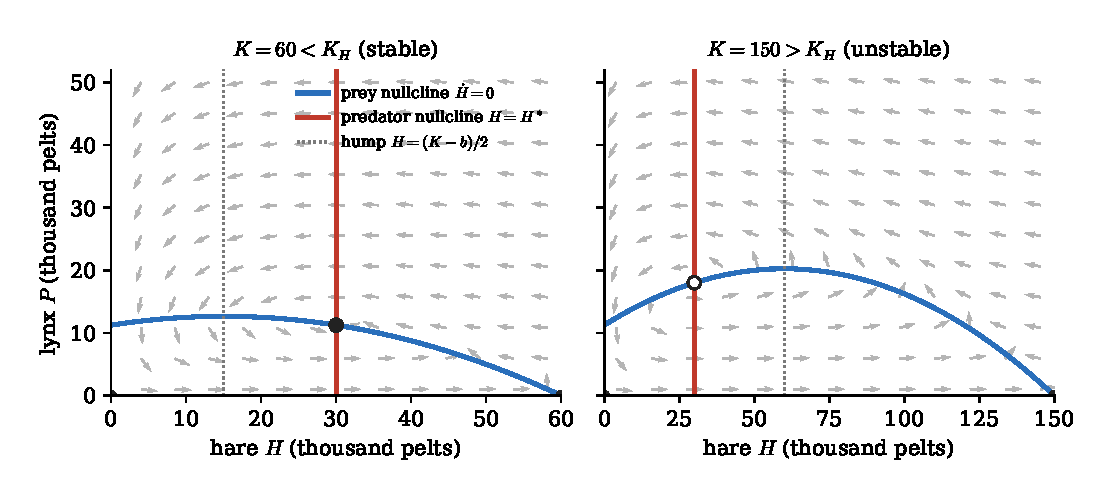
\includegraphics[width=\linewidth]{joel_nullclines}
\caption{Nullclines and direction field for the illustrative parameters
($r=1.5,\ a=4,\ b=30,\ e=0.4,\ m=0.8$; $H^*=30$, $K_H=90$).
Left: $K=60$; the predator nullcline meets the parabola right of its hump and $E^*$ (filled)
is a stable focus. Right: $K=150$; the intersection is left of the hump and $E^*$ (open) is
unstable. Small dots mark $E_0$ and $E_1$.}
\label{fig:nullclines}
\end{figure}

% ---------------------------------------------------------------------
\subsection{Hopf bifurcation with $K$ as the parameter}\label{sec:joel-hopf}

We fix $r,a,b,e,m$ with $ea>m$ and vary $K$ over $(H^*,\infty)$. Note $H^*$ is independent of
$K$, while $P^*$ increases with $K$.

\begin{theorem}[Hopf bifurcation]\label{thm:hopf}
At $K=K_H=b+2H^*$ the coexistence equilibrium undergoes a Hopf bifurcation:
\begin{enumerate}
\item[(i)] $\tau(E^*)=0$ and $\Delta(E^*)=\dfrac{rmb\,(K_H-H^*)}{K_H(b+H^*)}=\dfrac{rmb}{K_H}>0$,
so $J(E^*)$ has eigenvalues $\pm i\omega_0$ with
\[
\omega_0=\sqrt{\frac{rmb}{b+2H^*}},\qquad T_0=\frac{2\pi}{\omega_0};
\]
\item[(ii)] (transversality) the real part of the eigenvalues, $\tau/2$, crosses zero with
nonzero speed:
\[
\frac{d}{dK}\Bigl(\frac{\tau}{2}\Bigr)\Big|_{K=K_H}=\frac{rH^*}{2(b+H^*)(b+2H^*)}>0 .
\]
\end{enumerate}
\end{theorem}

\begin{proof}
(i) Substitute $K=K_H$ into~\eqref{eq:trace} and~\eqref{eq:det}; $K_H-H^*=b+H^*$ simplifies $\Delta$.
(ii) Differentiate~\eqref{eq:trace} in $K$: $\frac{d}{dK}\frac{K-K_H}{K}=\frac{K_H}{K^2}$, which equals
$1/K_H$ at $K=K_H$. All symbolic steps were checked with SymPy (\texttt{scripts/joel\_symbolic\_derivation.py}) and the closed forms are tested against the shared model code (\texttt{tests/test\_stability.py}).
\end{proof}

Conditions (i)--(ii) establish that a pair of complex eigenvalues crosses the imaginary axis.
To conclude that a small periodic orbit is born, and on which side, the Hopf theorem also needs
the first Lyapunov coefficient $\ell_1$ to be nonzero~\cite{kuznetsov2004}: $\ell_1<0$ gives a
\emph{supercritical} bifurcation (a stable cycle for $K>K_H$) and $\ell_1>0$ a subcritical one.

\paragraph{What is analytic and what is numerical.} We separate four statements.
\begin{enumerate}
\item \textbf{Analytic (derived here):} the threshold $K_H$, conditions (i)--(ii), and the
exchange of stability at $E^*$.
\item \textbf{Analytic (derived here): existence of a periodic orbit for $K>K_H$.}
Take any initial condition in the open quadrant. By Lemma~\ref{lem:bounded} its $\omega$-limit
set $\Omega$ is nonempty and compact. $\Omega$ cannot contain $E^*$, which is a repeller.
$\Omega$ cannot be $\{E_1\}$, because the stable manifold of the saddle $E_1$ is the $H$-axis.
If $\Omega$ contained $E_1$ together with other points, it would contain a point of $E_1$'s
stable manifold on the $H$-axis and hence the whole axis orbit through it, which tends backward
to $E_0$; repeating the argument at $E_0$ would put a point of the $P$-axis in $\Omega$, whose
backward orbit is unbounded, contradicting compactness. So $\Omega$ contains no equilibria, and
the Poincar\'e--Bendixson theorem~\cite{strogatz2015} makes $\Omega$ a periodic orbit.
\item \textbf{Cited theorems:} Cheng~\cite{cheng1981} proved the limit cycle is \emph{unique} for
$K>K_H$; since every interior orbit other than $E^*$ tends to a periodic orbit, that unique cycle
attracts them all and is orbitally stable. Hsu~\cite{hsu1978} proved that a locally stable $E^*$
is \emph{globally} stable in the open quadrant whenever the prey nullcline is concave, which our
parabola~\eqref{eq:prey-null} is, so $E^*$ attracts every interior orbit for $H^*<K<K_H$.
We use these results without reproducing their proofs.
\item \textbf{Numerical (for our parameter set only):} evaluating Kuznetsov's formula for
$\ell_1$ at $K=K_H$ gives $\ell_1\approx-4.0\times10^{-4}<0$ (and $-1.3\times10^{-3}$ for a second
set $r=0.7,\ m=0.5,\ b=20$), so the bifurcation is supercritical, consistent with the cited
uniqueness result. Simulations confirm the supercritical signature: the post-transient cycle
half-amplitude in $H$ scales as $(K-K_H)^{1/2}$ (fitted log--log slope $0.507$ for
$K-K_H\in[0.5,8]$), and the period tends to $T_0$.
\end{enumerate}

\noindent None of this says that the \emph{real} hare--lynx data sit on a limit cycle. That
depends on whether fitted parameters satisfy $K>K_H$, and with about two oscillations in
1900--1920 a slowly damped oscillation ($K$ slightly below $K_H$) can fit the same data.
That question belongs to the fitting sections and must be answered there with uncertainty.

\begin{figure}[ht]
\centering
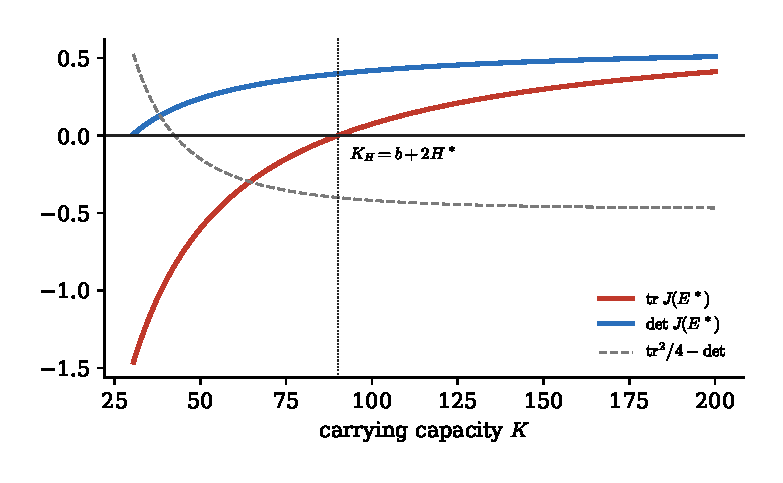
\includegraphics[width=0.7\linewidth]{joel_trace_det}
\caption{Trace and determinant of $J(E^*)$ as functions of $K$ (illustrative parameters).
The determinant stays positive for all feasible $K>H^*=30$, while the trace changes sign at
$K_H=90$. The dashed curve is negative (focus) for $K>42.5$.}
\label{fig:trace-det}
\end{figure}

% ---------------------------------------------------------------------
\subsection{The paradox of enrichment}

Increasing $K$ (enriching the hares' environment) leaves $H^*$ unchanged and only raises $P^*$:
every extra unit of carrying capacity is passed to the predator. Graphically, the prey parabola's
hump $(K-b)/2$ moves right while the predator nullcline stays at $H^*$, so for large enough $K$
the intersection falls left of the hump and the equilibrium destabilises. Past $K_H$ the system
settles on a limit cycle whose amplitude grows with $K$. For our illustrative parameters, at
$K=150$ the hare minimum on the cycle is about $1.1$ thousand, compared with $H^*=30$. In a
finite, stochastic population such deep troughs bring a real risk of extinction. Enrichment
thus \emph{destabilises} the system, the paradox named by Rosenzweig~\cite{rosenzweig1971}.

The mechanism is the saturating Holling type II response. At low $H$ each lynx's consumption
rises almost linearly with prey, which damps fluctuations; near and above $b$ it saturates, so
per-capita predation risk $aP/(b+H)$ \emph{falls} as hares increase. That positive feedback on
prey growth is exactly the term making $J_{11}>0$ left of the hump.

\paragraph{Link to Lotka--Volterra.} In the classical model ($K=\infty$, linear response) the
analogous Jacobian at coexistence has $\tau\equiv0$ for every parameter value, so it sits
permanently on the Hopf boundary. That is why its neutral cycles are structurally unstable: any
small change in the model's form moves it to one side or the other.
Rosenzweig--MacArthur makes the side explicit through the sign of $K-K_H$.

% ---------------------------------------------------------------------
\subsection{Illustrative regimes and numerical validation targets}\label{sec:joel-regimes}

These parameters are \emph{illustrative, not fitted}: $H$ and $P$ in thousands of pelts, $t$ in
years, with $r=1.5,\ a=4,\ b=30,\ e=0.4,\ m=0.8$. Then $ea=1.6=2m$, so $H^*=b=30$, $K_H=90$,
$\omega_0=\sqrt{0.4}\approx0.632$ and $T_0\approx9.94$ years, close to the observed decadal
cycle. Table~\ref{tab:joel-regimes} gives the expected behaviour on each side of the threshold;
the simulation section reproduces these with RK45 (\texttt{rtol}$=10^{-10}$,
\texttt{atol}$=10^{-12}$, 3000-year burn-in, start $(20,5)$).

\begin{table}[ht]
\centering
\small
\caption{Regimes in $K$ (other parameters fixed). Eigenvalues are of $J(E^*)$, except in A where
they are of $J(E_1)$.}
\label{tab:joel-regimes}
\setlength{\tabcolsep}{4pt}
\begin{tabular}{@{}cr l l l@{}}
\toprule
 & $K$ & Linear prediction & Eigenvalues & Long-run behaviour (simulated)\\
\midrule
A & 25  & $E^*$ infeasible ($K<H^*$) & $-1.5,\ -0.073$ & lynx die out; $\to(25,0)$\\
B & 60  & $E^*$ stable focus & $-0.188\pm0.515i$ & $\to(30,\,11.25)$, e-fold $\approx5$ yr\\
C & 85  & just below $K_H$ & $-0.022\pm0.623i$ & $\to(30,\,14.56)$, e-fold $\approx45$ yr\\
D & 90  & Hopf point & $\pm0.632i$ & very slow (algebraic) decay\\
E & 95  & just above $K_H$ & $+0.020\pm0.640i$ & cycle: $H\in[15.8,50.9]$, $P\in[9.8,20.8]$, $T=10.25$\\
F & 150 & well above $K_H$ & $+0.150\pm0.676i$ & cycle: $H\in[1.1,134.3]$, $P\in[1.7,41.2]$, $T=13.91$\\
\bottomrule
\end{tabular}
\end{table}

\noindent Two cautions for the numerics. At D the equilibrium is a weak focus ($\ell_1<0$), so
oscillations decay only like $t^{-1/2}$; after 3000 years the residual amplitude in $H$ is still
about $1.5$, which is expected and is not a sign of a cycle. The cycle at E is already large
because the amplitude coefficient is large ($A_H\approx7.8\sqrt{K-K_H}$), so ``small
amplitude'' only holds within about one unit of $K_H$.

\begin{figure}[ht]
\centering
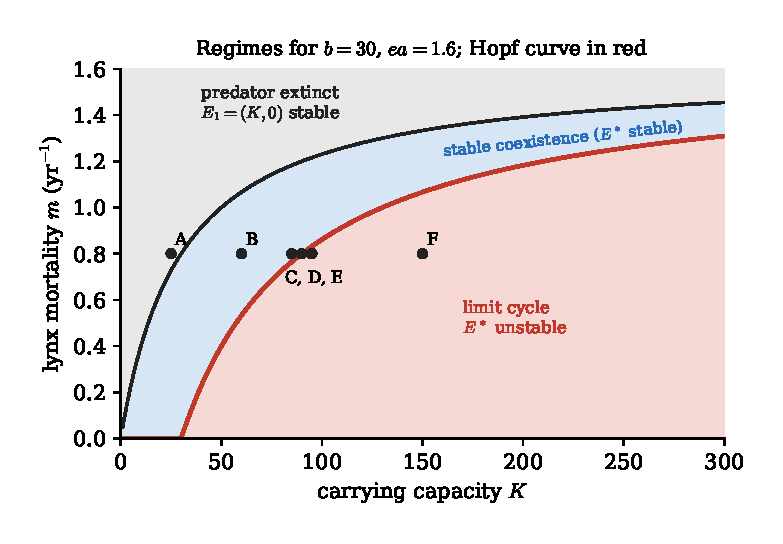
\includegraphics[width=0.7\linewidth]{joel_regions}
\caption{Analytic regimes in the $(K,m)$ plane for $b=30$, $ea=1.6$. Black curve:
$m=eaK/(b+K)$ (predator persistence boundary). Red curve: $m=ea(K-b)/(K+b)$ (Hopf curve).
Dots mark regimes A--F of Table~\ref{tab:joel-regimes}.}
\label{fig:regions}
\end{figure}

% ---------------------------------------------------------------------
\subsection{Sensitivity of the threshold}

Because $K_H=b(ea+m)/(ea-m)$ is explicit, sensitivity can be read off exactly. The elasticities
(percentage change in $K_H$ per percentage change in a parameter) are
\[
\frac{\partial\ln K_H}{\partial\ln b}=1,\qquad
\frac{\partial\ln K_H}{\partial\ln m}=-\frac{\partial\ln K_H}{\partial\ln a}
=-\frac{\partial\ln K_H}{\partial\ln e}=\frac{2\,ea\,m}{(ea)^2-m^2},\qquad
\frac{\partial\ln K_H}{\partial\ln r}=0.
\]
At the illustrative values ($ea=2m$) the middle elasticity is $4/3$: a 10\% rise in lynx
mortality raises the threshold by about 13\%, and so stabilises the system. The elasticity blows
up as $m\to ea$, where the predator is barely viable and $K_H\to\infty$. Weak predators stabilise.

Equivalently, for fixed $K$ the regimes are bands in $m$ (Figure~\ref{fig:regions}):
\[
\underbrace{m<\frac{ea(K-b)}{K+b}}_{\text{limit cycle}}
\qquad
\underbrace{\frac{ea(K-b)}{K+b}<m<\frac{eaK}{K+b}}_{\text{stable coexistence}}
\qquad
\underbrace{m>\frac{eaK}{K+b}}_{\text{lynx extinct}}
\]
A useful single number for any fitted parameter set is the \emph{stability margin}
$\sigma=K/K_H$: $\sigma<1$ means damped oscillations, $\sigma>1$ a limit cycle. Reporting
$\sigma$ (with its spread over fits) is the cleanest way to say whether the data support
sustained cycling.

Two structural facts matter for inference. First, $a$ and $e$ enter $H^*$, $K_H$ and the
stability conditions only through the product $ea$. Second, if lynx are measured only up to an
unknown multiplicative factor $c$ (as pelt counts are), the map $(P,a,e)\mapsto(cP,\,a/c,\,ec)$
leaves~\eqref{eq:rm} unchanged (checked symbolically), so $a$ and $e$ are \emph{not separately
identifiable} from index data. Fitting should fix one of them, or fit $ea$ and a scale, rather
than report both as biological rates.

% ---------------------------------------------------------------------
\subsection{Dimensionless form of the results}

With the scaling $x=H/K$, $y=aP/(rK)$, $s=rt$ (to be reconciled with the frozen scaling in the
model section), \eqref{eq:rm} becomes
\[
x'=x(1-x)-\frac{xy}{\beta+x},\qquad y'=y\Bigl(\frac{\alpha x}{\beta+x}-\delta\Bigr),
\qquad \beta=\frac{b}{K},\ \alpha=\frac{ea}{r},\ \delta=\frac{m}{r}.
\]
Then $x^*=\beta\delta/(\alpha-\delta)$, coexistence requires $\alpha>\delta$ and $x^*<1$, and the
Hopf condition $K=K_H$ reads $\beta(\alpha+\delta)/(\alpha-\delta)=1$, i.e.\ $\beta+2x^*=1$.
Only three combinations of the six parameters control the qualitative dynamics.

% ---------------------------------------------------------------------
\begin{table}[ht]
\centering
\small
\caption{Status of each stability claim in this section.}
\label{tab:joel-evidence}
\begin{tabular}{@{}p{0.52\linewidth}p{0.42\linewidth}@{}}
\toprule
Claim & Evidence \\
\midrule
Equilibria, feasibility, local stability of $E_0,E_1,E^*$ & Derived here; SymPy-checked\\
Hopf threshold $K_H=b+2H^*$, $\Delta>0$, transversality & Derived here; SymPy-checked\\
A periodic orbit exists for every $K>K_H$ & Derived here (Poincar\'e--Bendixson)\\
Cycle is unique and attracting for $K>K_H$ & Cited theorem~\cite{cheng1981}\\
$E^*$ globally stable for $H^*<K<K_H$ & Cited theorem~\cite{hsu1978}\\
Supercritical Hopf ($\ell_1<0$) & Numerical evaluation of analytic formula, two parameter sets\\
$\sqrt{K-K_H}$ amplitude law; periods, amplitudes, lags & Numerical (RK45), illustrative parameters\\
Real hare--lynx data lie on a limit cycle & \emph{Not established here}; requires $\sigma>1$ at fitted values with uncertainty\\
\bottomrule
\end{tabular}
\end{table}
